% THIS IS AN EXAMPLE DOCUMENT FOR VLDB 2012
% based on ACM SIGPROC-SP.TEX VERSION 2.7
% Modified by  Gerald Weber <gerald@cs.auckland.ac.nz>
% Removed the requirement to include *bbl file in here. (AhmetSacan, Sep2012)
% Fixed the equation on page 3 to prevent line overflow. (AhmetSacan, Sep2012)

\documentclass{vldb}
\usepackage{balance}  % for  \balance command ON LAST PAGE  (only there!)
\usepackage{graphicx}
\usepackage{cite}
\usepackage{caption}
\usepackage{subcaption}
\usepackage{alltt}
\usepackage[hidelinks]{hyperref}
\usepackage{algpseudocode}
\usepackage{algorithm}
\bibliographystyle{unsrt}
\usepackage{amssymb}
\usepackage[subtle]{savetrees}
\usepackage{amsmath}
\usepackage{booktabs}
\usepackage[table]{xcolor}
\usepackage{array}
\usepackage{pgfplots}
\usepackage{listings}     
\pgfplotsset{compat=1.13}


\newcommand{\KVS}{{\small \textsf{KV-store}}}
\newcommand{\KVSs}{{\small \textsf{KV-stores}}}
\newcommand{\HB}{{\small \textsf{HBase}}}
\newcommand{\TL}{\textsf{TL}}
\newcommand{\BT}{{\small \textsf{Bigtable}}}
\newcommand{\CAS}{{\small \textsf{Cassandra}}}
\newcommand{\DY}{{\small \textsf{Dynamo}}}
\newcommand{\PN}{{\small \textsf{PNUTS}}}
\newcommand{\VMS}{{\small \textsf{VMS}}}
\newcommand{\VMs}{{\small \textsf{VMs}}}
\newcommand{\VM}{{\small \textsf{VM}}}

\begin{document}

% ****************** TITLE ****************************************

\title{Dynamic Scalable View Maintenance in KV-stores}

% possible, but not really needed or used for PVLDB:
%\subtitle{[Extended Abstract]
%\titlenote{A full version of this paper is available as\textit{Author's Guide to Preparing ACM SIG Proceedings Using \LaTeX$2_\epsilon$\ and BibTeX} at \texttt{www.acm.org/eaddress.htm}}}

% ****************** AUTHORS **************************************

% You need the command \numberofauthors to handle the 'placement
% and alignment' of the authors beneath the title.
%
% For aesthetic reasons, we recommend 'three authors at a time'
% i.e. three 'name/affiliation blocks' be placed beneath the title.
%
% NOTE: You are NOT restricted in how many 'rows' of
% "name/affiliations" may appear. We just ask that you restrict
% the number of 'columns' to three.
%
% Because of the available 'opening page real-estate'
% we ask you to refrain from putting more than six authors
% (two rows with three columns) beneath the article title.
% More than six makes the first-page appear very cluttered indeed.
%
% Use the \alignauthor commands to handle the names
% and affiliations for an 'aesthetic maximum' of six authors.
% Add names, affiliations, addresses for
% the seventh etc. author(s) as the argument for the
% \additionalauthors command.
% These 'additional authors' will be output/set for you
% without further effort on your part as the last section in
% the body of your article BEFORE References or any Appendices.

\numberofauthors{3} %  in this sample file, there are a *total*
% of EIGHT authors. SIX appear on the 'first-page' (for formatting
% reasons) and the remaining two appear in the \additionalauthors section.

\author{
{\rm Jan Adler}\\
TU M\"unchen
\and
{\rm Martin Jergler}\\
TU M\"unchen
\and
{\rm Arno Jacobsen}\\
TU M\"unchen
}
% There's nothing stopping you putting the seventh, eighth, etc.
% author on the opening page (as the 'third row') but we ask,
% for aesthetic reasons that you place these 'additional authors'
% in the \additional authors block, viz.
\additionalauthors{Additional authors: John Smith (The Th{\o}rv\"{a}ld Group, {\texttt{jsmith@affiliation.org}}), Julius P.~Kumquat
(The \raggedright{Kumquat} Consortium, {\small \texttt{jpkumquat@consortium.net}}), and Ahmet Sacan (Drexel University, {\small \texttt{ahmetdevel@gmail.com}})}
\date{30 July 1999}
% Just remember to make sure that the TOTAL number of authors
% is the number that will appear on the first page PLUS the
% number that will appear in the \additionalauthors section.


\maketitle

\begin{abstract}
Distributed \textit{key-value stores} have become the solution of
choice for many data-intensive applications. However, their limited
query language support imposes challenges for applications that
require sophisticated query capabilities.  To address this problem, in
this paper, we develop the \textit{View Maintenance System} (\VMS) to
incrementally maintain selection, projection, aggregation, and join
views on behalf of applications.  We design \VMS\ given a generic
\KVS\ model based on a small number of features available in many
popular store architectures.  \VMS\ supports the maintenance of
hundreds of views in parallel, while simultaneously providing
guarantees for view consistency, even under node crash scenarios.  To
evaluate our concepts, we deliver a full-fledged implementation of
\VMS\ through Apache's \HB\ and conduct an extensive experimental
study. Exploiting parallel maintenance, \VMS\ achieve 
throughputs up to 60k view updates per second (120k table updates). 
\end{abstract}



\section{Introduction}
\label{sec:introduction}

%Context
Today's large scale internet services (e.g. Google Maps, Facebook, 
Amazon, etc.) handle millions of client requests, producing 
terabytes of data on a daily basis~\cite{parikh:facebook}. To handle 
this load, major internet companies have developed distributed 
databases called KV-stores such as Google's BigTable\cite{chang:bigtable},
Amazon's Dynamo~\cite{decandia:dynamo}, Yahoo's
PNUTS~\cite{cooper:pnuts}, Apache's HBase~\cite{george:hbase} and
Cassandra~\cite{hewitt:cassandra} (originally Facebook).

KV-stores are highly available to the user and provide advanced 
features like automated load balancing and fault tolerance. KV-stores 
scale horizontally -- by partitioning data and request load across a 
configurable number of nodes. To achieve these properties at a large-scale, 
KV-stores sacrifice an expressive query language and data model, only 
offering a simple API, comprising of \textit{put}, \textit{get} and 
\textit{delete} operations. While this API provides efficient access 
to single row entries, the processing of more complex (SQL-like) queries, e.g. 
selection, aggregation, and join, require costly application-level 
operations. Although, some KV-stores provide additional features to 
support higher-level query processing, those features are often 
rudimentary and impose bottlenecks. 

 Many existing approaches separate transactional and analytical 
processing. A complete snapshot of the data base is copied or loaded to 
an \textit{external} data warehouse and then, processed in a batch-wise 
fashion. Therefore, numerous existing frameworks with varying 
abstraction levels are available, e.g. Map Reduce \cite{dean:mapreduce}, 
Apache Spark \cite{zaharia:spark}, Apache Hive \cite{thusoo:hive}, etc. 
While this approach exploits the benefits of high performance parallel 
processing, it always requires an initial load overhead. Further it is 
not capable of providing up-to-date results -- as frequent changes in 
the base data occur. 

Another way of solving the problem is the use of \textit{internal} 
KV-store mechanisms that directly operate on the KV-store data. Apache 
Pheonix \cite{phoenix:apache} enables rich SQL 
semantics by using the coprocessor functionality (little code snippets, 
deployed on the KV-store nodes) of HBase. While this approach is 
implementation bound to a specific KV-store, we strive for a more general 
solution. 
 

Our approach introduces mechanisms for the materialization and 
incremental maintenance of views to KV-stores. The user 
attains sophisticated query capabilities, simply through definition of 
view expressions. The KV-store keeps results highly available and
enables access of many clients in parallel -- as materialized views 
are simple tables managed in KV-store. Likewise, views can be maintained 
incrementally; only those view records are updated whose 
base records have been changed. The challenge then, is not the scanning
 and computation of base data any more, but the efficient and correct 
maintenance of views. To achieve this at scale, we develop the 
\textit{Distributed View Maintenance System} (VMS) as shown in 
Figure~\ref{fig:research_goal}. The VMS consumes streams of client 
operations (of a base table) and produces the corresponding updates 
(to the view table). 

\begin{figure} 
	\centering 
	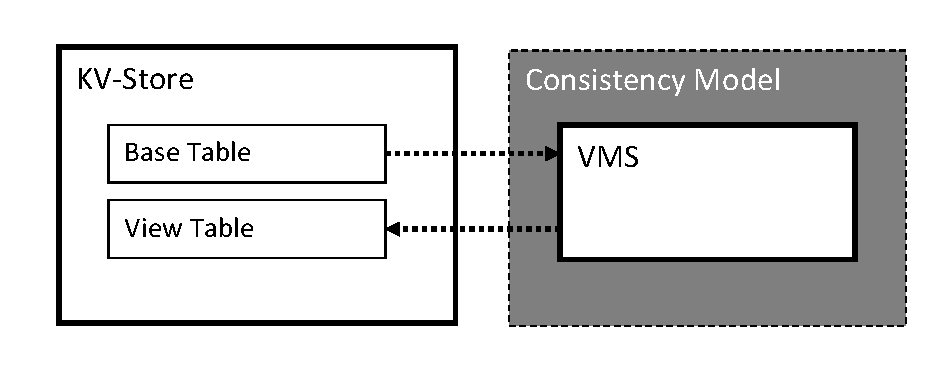
\includegraphics[width=\linewidth]{figures/ResearchGoal} 
	\vspace{-10mm} 
	\caption{System overview} 
	\vspace{-5mm} \label{fig:research_goal} 
\end{figure} 

First, we examine a set of KV-store 
implementations\cite{george:hbase, 
hewitt:cassandra, chang:bigtable, cooper:pnuts} and derive the common 
key characteristics from their architectures and their data models 
(Section~\ref{sec:kv_model}). As is common in the literature on view 
maintenance, we use a consistency model 
(Section~\ref{sec:consistency}) to ensure materialized views remain 
consistent with base data. But unlike the existing 
models\cite{zhuge:view, wang:efficient, zhang:parallel} -- which where 
mainly applied to centralized data warehouse environments -- we design 
our own consistency model to match the needs of a highly distributed 
environment (i.e. KV-stores). Based on the KV-store model and the requirements
of the consistency model, we describe 
the design of the scalable VMS (Section~\ref{sec:view_maintenance_system}). 
We design our VMS to scale in view update load and number of views 
maintained. Our design does not interfere with the read/write processing 
against tables in the KV-store, thus, leaving base table processing 
latencies unaffected. Finally, we conduct a comprehensive 
experimental study (Section~\ref{sec:evaluation}).

% Our approach integrates ``naturally'' with the 
%KV-store: Materialized views are simply tables managed by the store. In 
%spirit with the design philosophy of KV-stores, our approach resorts to 
%incremental and asynchronous view maintenance~\cite{gupta:maintaining, 
%lee:efficient, salem:how}. 

%The VMS is based on the properties and architecture of a typical 
%KV-store -- such as BigTable, HBase, Cassandra, and PNUTS.  



%The correct materialization of views, despite asynchronous and
%concurrent operation processing, is a major concern in the design of VMS.



%That is, only those parts of view tables that 
%are effected as base data changes, are updated. Base updates are 
%propagated asynchronously, not introducing new, costly control 
%dependences into the system. design of our view.  


%We develop a general KV-model in Section~\ref{sec:kv_model}. We adapt
%an existing consistency model in Section~\ref{sec:consistency}. We describe
%the design and behaviour of our View Maintenance System in 
%Section~\ref{sec:view_maintenance_system}.
%our approach.

%Update schema
%Furthermore, we develop a view materialization scheme that avoids 
%expensive table scans and related consistency issues in 
%Section~\ref{sec:view_maintenance}. Our approach supports the 
%maintenance of \texttt{SELECTION}, \texttt{PROJECTION}, \texttt{INDEX}, 
%aggregation (e.g., \texttt{COUNT}, \texttt{SUM}, \texttt{MIN} and 
%\texttt{MAX}), and general \texttt{JOIN} views. To achieve this, we 
%introduce a number of auxiliary view types, such as the \texttt{DELTA}, 
%\texttt{PRE-AGGREGATION} and \texttt{REVERSE-JOIN} view, which are 
%designed to support fast and efficient view maintenance. 



%The correct materialization of views, despite asynchronous and
%concurrent update processing, is a major concern in the design of VMS.
%As is common in the literature on view maintenance, we are using a
%consistency model to ensure materialized views remain consistent with
%base data.  But unlike the existing models\cite{zhuge:view,
%  wang:efficient, zhang:parallel} --- which where mainly applied to
%centralized data warehouse environments --- we design our own consistency
%model in Section~\ref{sec:consistency}, which matches the needs of a 
%highly distributed environment (i.e.  KV-stores). Subsequently, we
%analyse our VMS with regard to the model. While scaling up to hundreds 
%of nodes, fault tolerance becomes a big issue in any distributed system. 
%Thus, we discuss the steps of automatic recovery after crashed components 
%in Section~\ref{sec:fault_tolerance}. Finally, we evaluate our work in 
%Section~\ref{sec:evaluation}, given a 
%full-fledged implementation of the presented concepts based on Apache 
%HBase.  We conduct a comprehensive experimental study that evaluates 
%our approach.


%
\section{Background}

In \cite{adler_vms}, we showed how materialized views can be
incrementally maintained in a KV-store. Therefore, we developed
an architecture called VMS (cf. Figure~\ref{fig:system_overview}).
Now, we briefly explain the architecture necessary to create and
update view tables in a KV-store.


At the top of Figure~\ref{fig:system_overview}, a general KV-store 
architecture is depicted. It has been derived by looking at various
KV-store implementations (\cite{kv_store1, kv_store2, kv_store3, 
kv_store4, kv_store5}). A KV-store usually comprises a scalable set
of data nodes, each hosting a part of the overall data.  

In Figure~\ref{fig:system_overview} the first node is magnified such that
the write path of the system can be observed. When a client update 
comes in, the client is routed to an appropriate node (e.g. Node~1).
Then, the \textit{client operation} -- in a KV-store it is either a put 
or a delete -- is written to a \textit{transaction log} (TL). The TL
is located on disk and, thus, our extension component (cf. Figure~
\ref{fig:system_overview}) is able to stream the operations from it,
asynchronously. As the figure shows, each node in the KV-store
possesses a TL and an extension component. 


\subsection{KV store}

A KV-store usually  


\begin{figure}[h!] 
	\centering 
	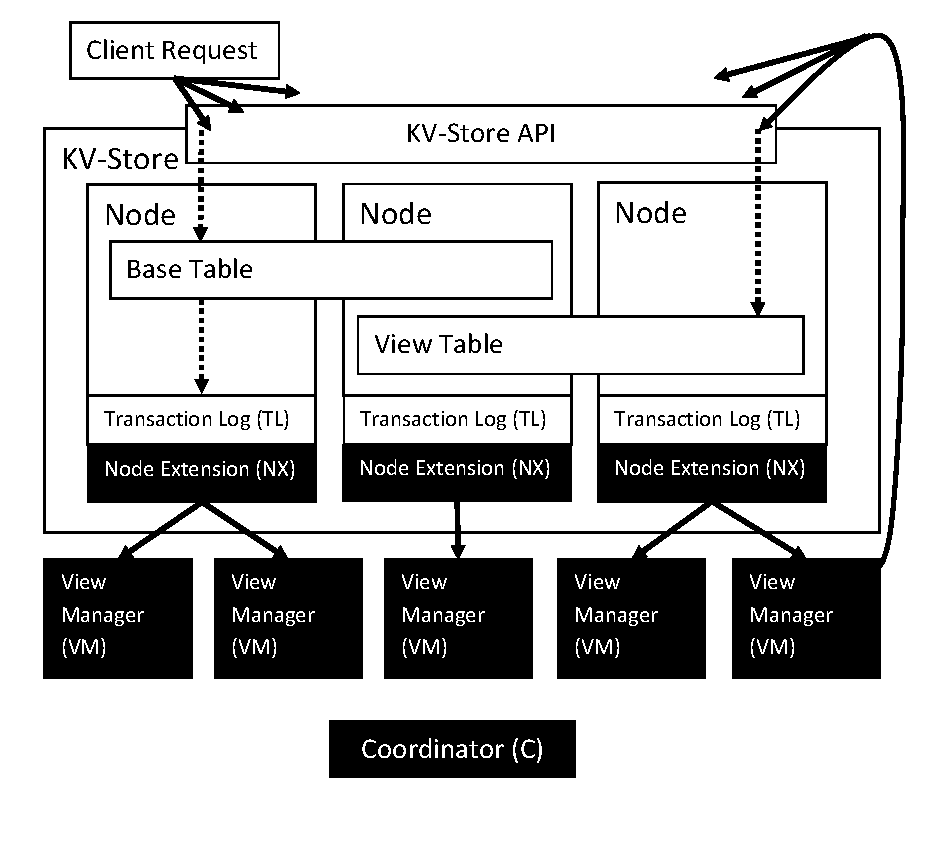
\includegraphics[width=\linewidth]{figures/SystemOverview}  
	\caption{System Overview} 
	\label{fig:system_overview} 
\end{figure} 





The View Maintenance System receives updates from the KV-store in form
of operation streams (see Figure~\ref{fig:system_overview}). Every node
of the KV-store produces a local transaction stream ($ts_1,..,ts_n$);every 
stream of operations is handled by a subsystem of the VMS. The subsystem 
parallizes view update computation: it distributes the updates to a
scalable number of view managers. A view manager actually applies the
update operation to the view table. First, it looks up the view tables 
 defined over the base, then it retrieves the corresponding view record, 
adds the delta to it, and writes back the result to the view.

We express view tables in the VMS with the help of relational algebra 
(e.g., we define a \texttt{SELECTION} as $S=\sigma_{c_1 < x}(A)$ over a 
base table $A$). Defining a view table over a base table is equivalent
to connection the output stream of base table operations with the input
stream of view table input operations. The VMS is also capable of 
defining view tables over view tables (e.g. we define a \texttt{PROJECTION}
view as $P=\pi_{c_1,c_2}(S)$). Thus,
we can concatenate multiple different view types; the VMS will update the
view chain subsequently. It will receive the base table update, apply the
update to the \texttt{SELECTION} view, and apply the result of the first
update to the \texttt{PROJECTION} view.
%
\section{View Maintenance System} 
\label{sec:view_maintenance_system} 

In this section, we present and discuss the design of \VMS. By
illustrating how a base table operation may effect a view table, we
provide the intuition for the resulting view consistency established
by \VMS.  Finally, we discuss fault-tolerance.

\subsection{Design Overview}

The lower half of Figure~\ref{fig:kv_model} gives an overview of \VMS, 
which is comprised of a \textit{master}, a number of $n$ 
\textit{source systems} (always the same number as \KVS\ nodes) and
a number of $m$ view manager. The 
input to \VMS\ is a set of operation streams; each emitted by a \KVS\ 
node (cf. Figure~\ref{fig:kv_model}). Technically, the \textit{WAL 
reader} component of a source system connects to the underlying HDFS and 
reads the WAL of its assigned node. Because operations are always 
appended to the WAL, the reading happens fast and in-order. After 
retrieving the operations from WAL, the WAL reader passes them to the 
distributor. This component distributes the incoming operation stream to 
all registered \VMs. The number of \VMs\ is configurable. \VMs\ can be 
dynamically \textit{assigned} to or \textit{removed} from the \VMS. 


A \VM\ is designed to be light-weight and can be deployed in large
numbers to accommodate a changing view update load. It computes view
updates, based on base table operations it receives as input via the
\KVS\ API, for view tables. A \VM\ only belongs to a single
sub-system. The sub-system feeds the \VM\ with operations which
processes them in order.  A \VM\ is the unit of scalability of
\VMS. \VMs\ are kept stateless to be exchangeable at any time and to
minimize dependency. Given a number of view definitions and a sequence
of operations, a \VM\ is always able to execute any view table update
from any host.

Our design exhibits at least the following four benefits: (i) Seamless
scalability: Hundreds of views may have to be updated as a consequence
of a single base table operation. As \VMS\ exceeds its service levels,
additional \VMs\ can be spawned (below, we show this
experimentally). (ii) Operational flexibility: \VMs\ introduce
flexibility to the system architecture. All \VMs\ of a given
sub-system can be hosted together on the same node or each \VM\ can be
hosted at a different node. (iii) Accommodate load variations:
\VMs\ can be reassigned from one sub-system to another as base table
update load changes. (iv) Fault-tolerance: If a \VM\ crashes, another
\VM\ can take over and continue processing the operation stream.

\subsection{Update Propagation} 
\label{subsec:update_processing} 

A source distributes the arriving base table updates (i.e. WAL stream) 
to the \VMs\ via consistent hashing by maintaining a hash-ring
(cf. Figure~\ref{fig:review_consistency}), where active \VMs\ are
registered.  Row keys of arriving updates are hashed into the ring and
associated in clock-wise direction with active \VMs.  In this way, a
source-system distributes operations uniformly across the available
\VMs\ and ensures that base table operations on the same row key are
always handled by the same \VM. On the one hand, this mechanism
ensures maximal degree of concurrency for update propagation, on the other
hand it guarantees the ordered propagation of base table
updates to view tables, setting the basis for view table consistency.

There are two alternatives to compute a the hash value of an update 
operation. \textit{Alternative~1:} the distributor component uses the 
hash of the base table row-key to determine a \VM\ (row-key k, cf. 
Figure~\ref{fig:review_consistency}). \textit{Alternative~2:} the 
distributor component uses the hash of the view table row-key to 
determine a \VM\ (row-key x, cf. Figure~\ref{fig:review_consistency}). 
If base table and view table have the same row-key (e.g. a selection 
view), both alternatives will match the same result. But if row-keys are 
different (e.g. an aggregation or join view), both alternatives will 
lead to different up- and downsides, which will be discussed in 
Subsection~\ref{sec:consistency}. 


Every \VM\ maintains its own transaction log, referred to as
\textit{\VM-log}. When receiving an operation, a \VM\ directly writes
it to the \VM-log. Just like the transaction log, the \VM-log is kept
available by the underlying file system, employing recovery mechanisms
in face of \VM\ crashes (e.g., in the case of \HB, the file system
redundantly replicates file blocks via HDFS.)

To access and update view tables, a \VM\ acts as a client to the \KVS,
using its standard client API. Given a base table operation (e.g., a
put on a base table $A$), the \VM\ retrieves and caches the view
definitions of the derived views (e.g., a \texttt{SELECTION} and
\texttt{COUNT} view $S$ and $C$, both derived from $A$). Then,
\VM\ runs the update program, and submits view table updates (to $S$
and $C$) via the client API. For some of the view types maintained,
the \VM\ has to query the view table first, as part of the update
logic; in a \texttt{COUNT} view, the \VM\ reads the current count from
the view before applying the delta of the base table operation. These
view queries are always get operations (i.e., single row accesses) and
can be evaluated quickly.



\begin{figure}
  \centering
    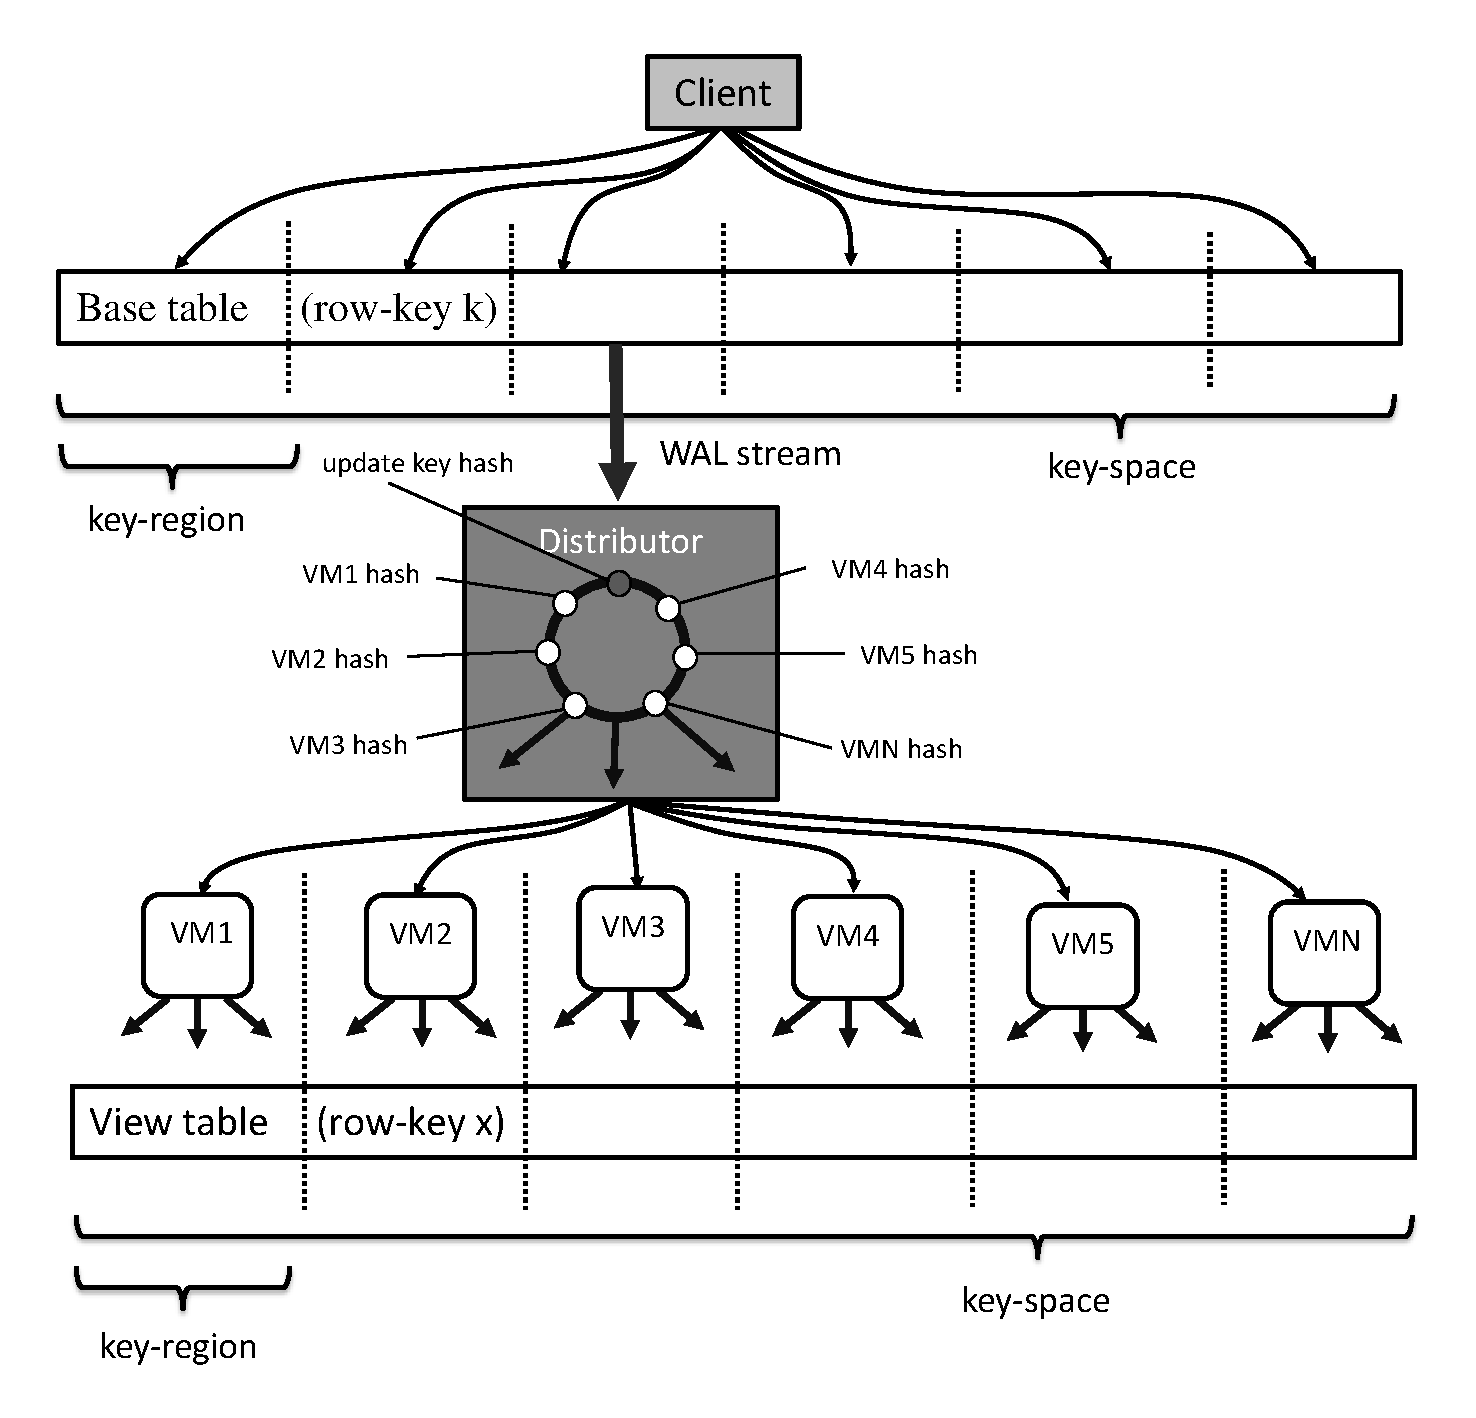
\includegraphics[width=\linewidth]{figures/Consistency}
    \caption{Update distribution through Consistent Hashing}
    \label{fig:review_consistency}
    \vspace{-2mm}
\end{figure}


%\subsubsection{Management Actions and Consistency} 
%
%We now refine the behaviour of \VMS\ to allow for dynamic state
%changes in sub-systems.  For reasons of recovery, load balancing and
%scaling, \VMS\ performs the following actions: \textit{add}, makes the
%\VM\ resource available to the \VMS; \textit{remove}, takes away a
%\VM\ resource; \textit{assign}, makes a \VM\ available to a sub-system
%such that it can process the sub-system's client operations;
%\textit{withdraw}, takes away a \VM\ from a sub-system (opposite of
%assign); and \textit{re-assign}, re-locates a \VM\ from one sub-system
%to another. Adding a \VM\ to \VMS\ (or removing it) does not affect
%view maintenance. The re-assign action is a combination of withdraw
%and assign. Now, we explain how assign and withdraw actions are
%performed safely (i.e., without interfering with consistency).
%
%%\begin{table}
%%\rowcolors{2}{gray!10}{gray!30}
%%\setlength{\belowrulesep}{0pt}
%%\setlength{\aboverulesep}{0pt}
%%\setlength\extrarowheight{2pt}
%%\begin{center}
%%\begin{tabular}{l l l}
%%\toprule
%%Component & action & method \\
%%\midrule
%%View Manager & add & \textit{addViewManager()}  \\
%% & remove & \textit{removeViewManager()}    \\
%% & assign & \textit{assignViewManager()}  \\
%% & withdraw & \textit{withdrawViewManager()}    \\
%% & re-assign & \textit{reassignViewManager()}    \\
%%\bottomrule 
%%\end{tabular}
%%\caption{\VMS\ actions}
%%\label{tab:vms_events}
%%\end{center}
%%\end{table}
%
%%Recall, that the sub-system selects the 
%%responsible \VM\ by applying the hash function. The operation is then 
%%inserted into the corresponding queue. 
%
%
%\noindent
%\textbf{Assign VM:} Figure~\ref{fig:review_consistency} shows how a
%sub-system does view maintenance. Assume a new \VM\ (in the figure
%represented by $V_3$) is assigned to the sub-system. The logic,
%performed on the sub-system during the command, can be described as a
%sequence of primitive actions: (1) Method $createQueue(vm)$ creates a
%queue for a new \VM. (2) The \VM\ is added to the hash-ring by method
%$insertHash(vm)$.  (3) The method $activateQueue(vm)$ starts the
%sending thread that keeps transferring the queue's operations to the
%\VM.
%
%When a \VM\ is assigned, it is inserted into the hash-ring of the 
%sub-system. Unless the hash-ring is empty, the new \VM\ is assigned a key 
%range that is, at the same time, removed from another \VM. This leads
%to violation of consistency (even convergence in terms of the consistency
%model), as the following example shows.
%
%
%\begin{algorithm}
%\caption{Safe assignment procedure at sub-system}
%\label{alg:assignvm}
%\begin{algorithmic}
%\Procedure{$assignVm$}{$vm_a, VM_{sub}$}
%\State{$createQueue(vm_a)$}
%\State{$insertHash(vm_a)$}
%\ForAll{$vm \in VM_{sub}$}
%\State{$queue(vm, m_a)$}\Comment{queue markers}	
%\EndFor
%\ForAll{$vm \in VM_{sub}$}
%\State{$receiveAck(vm)$}\Comment{wait for acks}		
%\EndFor
%\State{$activateQueue(vm_a)$}	
%\EndProcedure
%\end{algorithmic}
%\end{algorithm}
%
%
%\textit{Example}: In Figure~\ref{fig:review_consistency}, $VM_1$ and
%$VM_2$ are already assigned to the sub-system. They are responsible
%for a certain range on the hash-ring; queues are feeding them with
%incoming client operations. Assume a client performing a put operation
%$p_1(k_1, \{..\})$; the sub-system receives $p_1$, selects $VM_2$ as
%responsible and inserts $p_1$ into the queue of $VM_2$.  Now assume, a
%new \VM\ $VM_3$ is assigned to the sub-system and its hash is inserted
%within the range of $VM_2$ such that it acquires the responsibility
%for key $k_1$. In a next step, a client sends an operation $p_2(k_1,
%\{..\})$ to the same key. Because responsibility has changed, the
%operation is sent to $VM_3$. Considering that $VM_3$ has just been
%added, it's queue is empty and, hence, processes updates very fast. It
%is likely to happen that $VM_3$ processes $p_2$ before $VM_2$ can
%process $p_1$. Because both operations refer to the same base record,
%the timeline of the record is broken and convergence is violated.
%
%To process the assign command safely, we use so called \textit{markers}. 
%Markers are -- just like client operations -- enqueued to a \VM\ and 
%become a part of the operation stream. When the \VM, while processing 
%operations, notices a marker, it replies with an acknowledgement back to 
%the sub-system. Thus, the marker reveals to the sub-system, whether the \VM\ 
%has completed all operations that were sent before the marker. We change the 
%assignment procedure by adding a marker-based acknowledgement mechanism 
%(cf. Algorithm~\ref{alg:assignvm}). 
%
%%The
%%algorithm is executed synchronously and if another assignment
%%procedure is called on the sub-system, it must wait, until the first
%%operation has terminated.
%The procedure $assignVm$ takes two parameters: $vm_a$, the \VM\ that 
%should be assigned to the sub-system, and $VM_{sub}$, a set of \VMs\ 
%that are already assigned to the sub-system. The algorithm creates a 
%queue for $vm_a$ and inserts it into the hash-ring. Then, it queues a 
%marker $m_a$ to all assigned \VMs\ ($VM_{sub}$). After the sub-system 
%has received acknowledgements from all \VMs, it is guaranteed that no 
%operation in the key range of the newly added \VM\ $vm_a$ is still 
%pending. Referring back to the above example: The timeline of $k_1$ can 
%not be changed any more. 
%
%%Operation $t_2$ has to
%%wait in the queue of $VM_3$ until $VM_2$ acknowledges the processing
%%of $t_1$ because the queue of $VM_3$ is activated only after the
%%marker has been acknowledged and this, in turn, implies that operation
%%$t_1$ has been processed.
%\noindent
%\textbf{Withdraw VM:} The logic, performed on the sub-system side
%during a withdraw can be described analogously to the assign command
%by a sequence of primitives (opposite actions in reverse order): (1)
%$deactivateQueue(vm)$ stops the sending thread that keeps transferring
%the operations in the queue to the \VM. (2) The \VM\ is removed from
%the hash-ring by $removeHash(vm)$. (3) $deleteQueue(vm)$ removes the
%queue for the withdrawn \VM. The queue can only be deleted, if it is
%empty and no operation is queued.
%
%\begin{algorithm}
%\caption{Safe withdraw procedure at sub-system}
%\label{alg:withdrawvm}
%\begin{algorithmic}
%\Procedure{$withdrawVm$}{$vm_w, VM_{sub}$}
%\ForAll{$vm \in VM_{sub} \wedge vm \neq vm_w$}	
%\State{$deactivateQueue(vm)$}
%\EndFor
%\State{$removeHash(vm_w)$}
%\State{$queue(vm_w, m_w)$}\Comment{queue marker}
%%\ForAll{$vm \in VM_{sub}$}
%\State{$receiveAck(vm_w)$}\Comment{wait for ack}		
%%\EndFor
%\State{$removeQueue(vm_w)$}
%\ForAll{$vm \in VM$}
%\State{$activateQueue(vm)$}
%\EndFor
%\EndProcedure
%\end{algorithmic}
%\end{algorithm}
%
%    
%Also, during a withdraw procedure, consistency may be violated. At the
%moment where a \VM\ is withdrawn, i.e., removed from the hash-ring,
%its queue might still contain operations. If another \VM\ that
%acquires the key range is fast enough, it might processes operations
%before the withdrawn \VM\ has finished. Again, the timeline of base
%records is changed. In order to prevent inconsistencies, we designed
%Algorithm~\ref{alg:withdrawvm} analogously to
%Algorithm~\ref{alg:assignvm}. It takes two parameters: $vm_w$, the
%\VM\ that should be withdrawn from the sub-system, and $VM_{sub}$, the
%set of \VMs\ that is assigned to the sub-system.
%
%First, the queues of the \VMs\ that possibly increase their key range
%on the hash-ring (i.e., all other \VMs) are deactivated. Then, a
%marker $m_w$ is queued at the \VM\ that is withdrawn. If the \VM\ has
%acknowledged the marker, the sub-system knows, that all operations
%have been processed. It removes the queue of the \VM\ and re-activates
%the queues of all \VMs.
%

\subsection{Consistency}
\label{sec:consistency}

Since consistency is a major concern during incremental view maintenance 
-- additionally, we introduce a high degree of concurrency -- we now 
show, how the fundamentals of Section~\ref{subsec:consistency_model} 
influence the \VMS\ design. As a first step, we discuss the three rules
of Theorem~1, separately.


%we define a consistency model before building the VMS. 
%In data warehouse environments, for batch-based view update
%processing, consistency models have been extensively explored (e.g.,
%~\cite{zhuge:view, wang:efficient, zhang:parallel, zhuge:strobe}. For
%view maintenance in KV-stores a model has been proposed
%in~\cite{jacobsen:viewmaintenance}. First, we adapt this model and the
%corresponding consistency levels to match the characteristics of 
%KV-stores (defined in the previous section). Second, we define a theorem, 
%capturing the requirements against our VMS, in order to achieve strong
%consistency.



\subsubsection{Exactly once property}
\label{subsubsec:exactly_once}  

Like stated in our theorem, Rule~1, updating a view exactly once for 
every client operation is critical, as views can be non-idempotent. 
There are two possible incidents that 
violate the exactly once requirement: an operation is lost (maybe due to 
node crash, or transmission errors); an operation is applied 
more than once (in consequence of a log replay after a node crash). 
In either case, the view would be incorrect (i.e., does not converge).

One architectural decision of VMS was to read the update operations from
the WAL of the \KVS\ node. Updates in the WAL are persisted safely and
replicated via HDFS. Even though a node or a \VM goes down and update 
operations are lost, they can be always recovered from the WAL of the 
\KVS\ node. Actually, the WAL serves the same purpose for the \KVS\ itself.
As soon as a node crashes, the \KVS replays all transactions that have 
not been flushed to the table file before and would have been lost otherwise.


As updates cannot be lost, the \VMS\ guarantees an at-most-once semantic.
Still, we need to assure that updates in \VMS\ are not duplicated. In case a crash 
occurs, the WAL reader may re-process some of 
the updates and send them to the \VMs\ a second time. Then, the \VM\ needs 
to identify the duplicate and drop it. We achieve the identification of
duplicates with the help of a global ID (i.e. signature); this ID can only 
be obtained from the \KVS, as the update operations originate from here. 
Our implementation builds on top of \HB, a global ID can be created by 
combining an operations sequence number and the node ID. This ID is delivered
with every update operation. The \VM\ just keeps track of the highest maintained
operation ID (this information can be stored into Zookeeper, as the system is 
fault-tolerant). If ever an operation with a lower ID is sent to the \VM, it 
identifies the duplicate and drops it.




\subsubsection{Atomic view record update}
\label{subsubsec:atomic_update} 

Like stated in our theorem, Rule~2, every view update has to be executed 
atomically. Regarding a view update, we rely on the semantics that are 
provided by \KVS. We assume (as it is the case for \HB\ and \CAS) that a 
single put or delete operation, e.g. $put(k_1, \langle c_1, x_1\rangle, 
\langle c_2, 10\rangle)$, is executed ACID compliant. Thus, a row update 
has to be atomic; the \KVS\ is not allowed to execute let's say 
$put(k_1, \langle c_1, x_1\rangle)$ and then $put(k_1, \langle c_2, 
10\rangle)$ later. 


Despite the single update operation (i.e. get/put), also the complete 
update process -- comprising of a get-operation to the old view record 
and a put/delete- operation to the new view record -- has to be ACID 
compliant. Most view types define a mapping from multiple base table 
records to a single view table record (e.g. aggregation). As shown in 
Example~2 different base table records may be propagated to different 
VMs, multiple VMs can concurrently update the same view record. 
Remembering the execution alternatives from 
Subsection~\ref{subsec:update_processing}, this problem has to be 
solved, differently. 




\noindent
\textbf{Alternative~1:} Distributing the update operation according to the
base table row-key means, there could be multiple \VM, updating one view
table row-key. For example put operations $put(k_1, \langle c_1, x_1\rangle, 
\langle c_2, 10\rangle)$ and $put(k_5, \langle c_1, x_1\rangle, \langle c_2, 
5\rangle)$ could be forwarded to different \VMs, still both \VMs have to
access row key $x_1$. To solve the problem, we use test-And-set methods to 
avoid interruption during updates. The \VM\ retrieves the old view record,
e.g. $(x_1, \langle c_{sum},20\rangle)$ and extracts one of the values (here,
it is the aggregation value $20$). When updating and writing back the new 
value, e.g. $25$, the \VM\ sends a test-and-set request to the server with
a test-value (here $20$). 


\noindent
\textbf{Alternative~2:} Distributing the update operation according to the 
hash of the view table row-key completely eliminates the need of further 
synchronization mechanisms. Every \VM\ is responsible for an equal amount
of view table records and, thus, for a part of the view table. As there is 
no ambiguity, \VMs\ can just use regular get and put/delete operations.


%\noindent
%\textit{Example~3:} Given base table $A(\underline{K}, F)$ and a \texttt{SUM} 
%view $S(\underline{X}, F)$, defined as $S=\gamma_{c_1,Sum(c_2)}(A)$. 
%Assume a client inserts two records into base table $A$. The KV-store writes the following 
%operations into the transaction log: $t_1=put(k_1,\{\langle 
%c_1,x_1\rangle,\langle c_2,a\rangle\})$ and $t_2=put(k_2, \{\langle 
%c_1,x_1 \rangle,\linebreak \langle c_2,b\rangle\})$. Let the VMS receive both 
%operations and process them in parallel. To perform view maintenance, 
%the VMS retrieves the corresponding old view records from the view 
%table. Since $S$ is a \texttt{SUM} view -- and $t_1$ and $t_2$ refer to 
%the same aggregation key $x_1$ -- the VMS retrieves the same view record 
%twice, e.g. $(x_1, \{\langle c_s, v_s\rangle\})$. In case of $t_1$ VMS 
%adds the delta $a$ to the view record; in case of $t_2$ VMS adds the 
%delta $b$. Then, the VMS writes the updated view records back to the 
%view table. Depending on which record is written first, the VMS 
%overwrites one update with the other. Say, VMS writes $(x_1, \{\langle 
%c_s, v_s+a \rangle\})$ to $S$; then it overwrites the result with 
%$(x_1,\{\langle c_s, v_c+b\rangle\})$. In consequence the delta $a$ is 
%missing in the view. The correct result should be $(x_1,\{\langle c_s, 
%v_s+a+b \rangle\})$. Therefore, atomic view updates are essential. 
%


%In our implementation, we use a test-and-set mechanism to solve this
%problem.~\footnote{In HBase a \texttt{checkAndPut} method is provided
%  to realize this mechanism. Most KV-stores offer a similar
%  abstraction.} When updating a table record, a caller sees (tests)
%whether a record has been concurrently modified between a read and an
%update.
%
%Revisiting Example~2, let $VM_2$ retrieve value $(x1, \{(col_1,
%a)\})$. Then, it computes $(x1,\{(col_1,a+c)\})$ trying to put the new
%value, while testing for the old value $a$. The test-and-set fails
%because the old record value changed concurrently to $a+b$. Thus,
%$VM_2$ fetches the updated value again and re-computes
%$(x1,\{(col_1,a+b+c)\})$. This time the test-and-set succeeds and the
%record is written.

\subsubsection{Record timeline}
\label{subsubsec:record_timeline} 

Record timeline means that sequences of operations on the same row key are not re-ordered 
when processed by VMS.  Again, a little example demonstrates the
importance of record timeline semantics.


\noindent
\textbf{Alternative~1:} Distributing the update operation according to the
base table row-key means, time-line of a record cannot be broken. All 
operations that touch a specific row-key will always be directed to the 
same \VM; they will be retrieved in-order,  sent to the \VM\ in-order and
updated in the view in-order.
%
%there could be multiple \VM, updating one view
%table row-key. For example put operations $put(k_1, \langle c_1, x_1\rangle, 
%\langle c_2, 10\rangle)$ and $put(k_5, \langle c_1, x_1\rangle, \langle c_2, 
%5\rangle)$ could be forwarded to different \VMs, still both \VMs have to
%access row key $x_1$. To solve the problem, we use test-And-set methods to 
%avoid interruption during updates. The \VM\ retrieves the old view record,
%e.g. $(x_1, \langle c_{sum},20\rangle)$ and extracts one of the values (here,
%it is the aggregation value $20$). When updating and writing back the new 
%value, e.g. $25$, the \VM\ sends a test-and-set request to the server with
%a test-value (here $20$). 


\noindent
\textbf{Alternative~2:} Distributing the update operation according to the 
hash of the view table row-key also creates a record timeline. But in 
contrast to Alternative~1, it is the timeline of the view table, which
bears the following consequences: As long as the view table record doesn't
change, updates to the same base table row-key are also forwarded to the 
same \VM.  As soon as an update modifies the view table row-key -- which means
the update touches two records in one view table -- the timeline
of the base table row-key could be broken. 

For that reason, we need a mechanism which prevents this scenario. We 
employ a buffer for update operations. But only for those updates, that 
change the view table key in question -- insert and delete operations, 
as well as update operations that don't change the key are processed 
just like before; matching this criterion, the update is inserted into the 
buffer, send to a \VM, where it causes the old entry to be deleted; 
it is, then, deleted from the buffer and passed to another \VM, where it 
causes the new entry to be inserted. If during that process, however, more
updates flow in 




\subsubsection{Conclusion}
\label{subsubsec:conclusion} 

In the previous sections, we described two alternatives and their implications.
Both alternatives have their up- and downsides. Alternative~1 supports the 
preservation of base record time-line, whereas Alternative~2 supports the 
concurrent access to the view table. Both alternatives are convenient consistency
concepts, in both cases the implementation needs to be complemented with
additional mechanisms (i.e. test-and-Set methods, update buffer) to achieve
strong consistency. 

Still, we favor Alternative~2 over Alternative~1. One reason is the fact that
Alternative~1 uses Test-And-Set methods. Even though it is a pessimistic locking
mechanism -- in contrast to optimistic locking, a view record is always accessible --
it is not suited well in our case \footnote{Actually, modern system try to avoid locking completely} 
for the following reasons: (1) If there is high contention, a lot of view updates have
to be repeatedly applied, (2) we have to use test-and-set for every view update,
despite of it being an insert, update or delete, which introduces overhead. 
In contrast, we choose Alternative~2 for the following reasons: (1) it is a 
locking-free alternative (most state-of-the-art transaction systems use locking-free
mechanisms). (2) The update buffer is only needed for a small fraction of update
operations (i.e. not for inserts, not for deletes, etc..). Thus performance overhead
is minimal.





\subsubsection{Nested constructions}
\label{subsubsec:nested_constructions} 

So far, we have only discussed the simple case, with one base and one view
table. As we strive for support of more complex constructs (i.e. SQL-like 
queries) in \VMS, we need to extend our design.

\begin{figure}
  \centering
    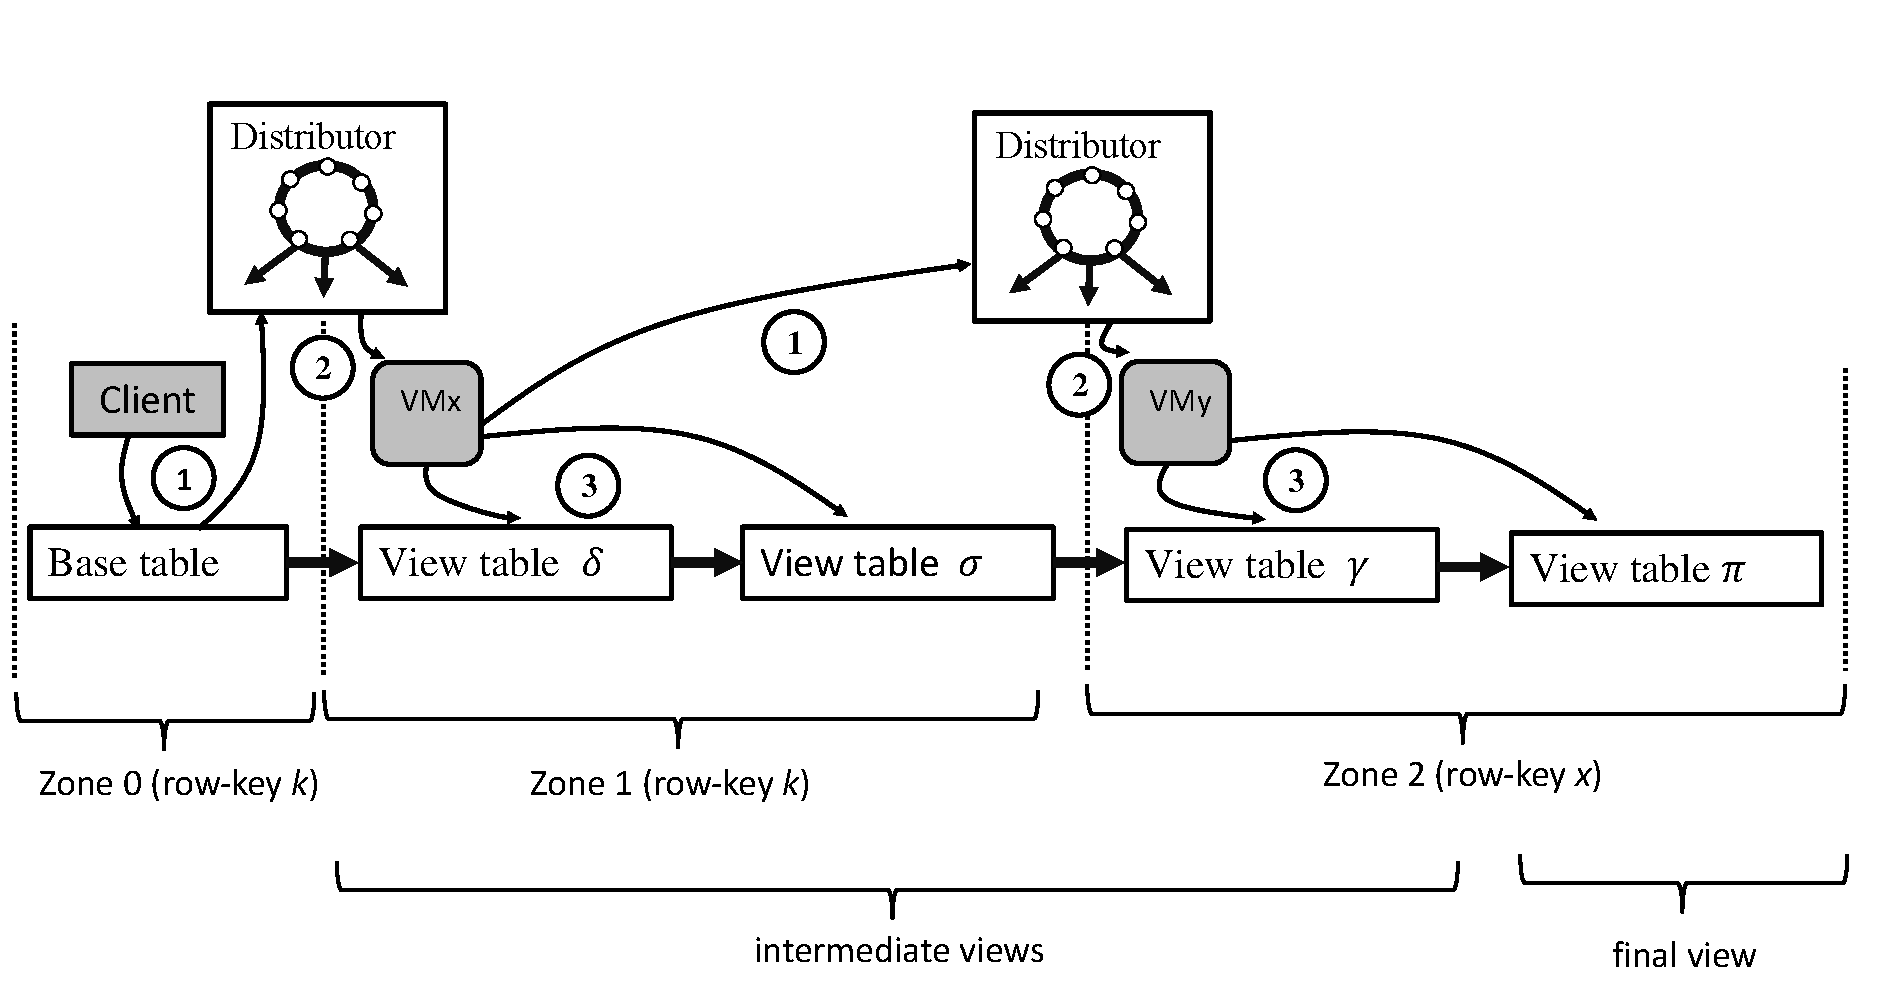
\includegraphics[width=\linewidth]{figures/Concept}
    \caption{Executing a query with views}
    \label{fig:view_concept}
    \vspace{-2mm}
\end{figure}

Usually, a query consists of multiple clauses (e.g. select, from, where, 
group by). In order to translate the query, we need to build a 
maintenance plan. This can be done with the help of a directed acyclic 
graph (DAG); each node in the DAG represents one materialized view. 
Starting from the base table, all views are inter-connected and each 
pair of view tables resembles a base/view table-relation. The moment a 
base table gets updated, the operation travels subsequently to all views 
and updates them incrementally. The result of the query can be obtained 
from the last view. 



In Figure~\ref{fig:view_concept}, the maintenance process of the 
following query is depicted: $\text{Select }sum(c2)\text{ from 
}bt1\text{ group by }c1\text{ where }c2\:<\:10$ It can be observed that 
the update path is divided into two \textit{zones}. A zone describes a 
part of the update path where all views possess the same row key. To improve
performance, a \VM\ can update the view tables of a zone in one run. 
Once a zone 
-- and therefore also the row key -- changes, updates need to be 
re-distributed in order to sustain consistency (cf. 
Figure~\ref{fig:review_consistency}). In the figure two zones can be 
identified. The maintenance of a zone is always processed in a cycle of 
three steps: 


\begin{enumerate}
	\item Update is provided to distributor
	\item Update is assigned and sent to VM
	\item Update is applied to view tables of zone
\end{enumerate} 


In the first step, the update operation is provided to the distributor
component of the source system. During maintenance of the first zone
the update is provided by the WAL reader of the source system itself, 
during maintenance of subsequent zones, it is provided by the last 
responsible \VM. In the second step, the distributor assigns and 
distributes updates as described above (cf. Figure~\ref{fig:view_concept}).
In the third step, the \VM\ goes along the path of each view table in
the zone, retrieves the old view record, updates it incrementally and 
stores the new version back into the view. Then the cycle is repeated
for every zone. As all the updates of a zone can are distributed 
according to the cardinality of the row key, a high parallelisation of 
updates can be achieved.


%\subsection{Proof of Consistency}


Theorem~\ref{theo:strong_consistency} states that a VMS system fulfilling all 
three requirements achieves at least strong consistency. In the following, we 
will present a proof for this theorem, which is organized in three stages: we 
start with proving convergence and then present extensions to also prove weak 
consistency  and finally strong consistency.





\subsubsection{Notation}
First, we define the following notation for keys, 
operations on keys, and the ordering of operations. Let $k_x$ denote a key in 
a base table, where $x \in X = \{1, \dots, m\}$, and $X$ is the 
table's key range. Further, let an operation on key $k_x$ be defined as 
$t[k_x]$, and a totally ordered sequence of such operations be denoted by 
$\langle t_1, t_2, t_{3}, \dots, t_N\rangle$, where $N$ defines the total 
number of operations on the table in a given timespan. 
Hence, a generalized sequence of operations on a base table is 
represented by $\langle t_1[k_{x_1}], t_2[k_{x_2}], \dots, 
t_n[k_{x_m}]\rangle$, where $k_{x_1}, \dots, k_{x_m} \in X$ can be arbitrarily 
chosen from the base table's key range for every timestamp. Based on this 
generalized sequence every other sequence of operations can be derived, e.g. 
$\langle t_1[k_{1}],t_2[k_{2}],t_3[k_{1}]\rangle$. In some cases, we also want 
to keep the ordering of operations variable. For that reason, we introduce an 
index $s_i$ with $i \in \{1, \dots, n\}$. Then we can write the arbitrary 
sequence as $\langle t_{s_1}[k_{x_1}], t_{s_2}[k_{x_2}], \dots, 
t_{s_n}[k_{x_n}]\rangle$ with $s_1\neq \dots \neq s_n$. Using this notion, we 
are capable of representing every possible sequence of update operations in 
the system. 

The index $t^{(i)}[k_x]$ is used to express a sequence of operations on 
a single row key (i.e. the time-line). For example, a sequence of 
operations on row key $k_x$ is denoted as $\langle 
t^{(1)}[k_x],t^{(2)}[k_x]...,t^{( \omega)}[k_x]\rangle$. The last 
operation on a particular row key is always denoted with $\omega$. (see 
Section~\ref{sec:consistency}).

For the proof, we assume such an arbitrary sequence of base table operations
 and then we show that --- given the requirements in the theorem --- a VMS 
 system will produce correct view results. Formally, we show that $V_f=View(B_f)$. 

\subsubsection{Convergence}
\label{sub:proof_convergence}
As mentioned earlier, every view type defines its own mapping from base table 
to view table records. Thus, we prove the different cases separately. 

\noindent
\textit{One-to-one mapping:} \texttt{SELECTION}, \texttt{PROJECTION} 
views define a one-to-one mapping between base and view table. The row 
key of the base table is also the row key of the view table. Operations 
for both view types are idempotent, meaning an operation could be 
applied several times without changing the result. The view record is 
always a representation of the last base table operation applied. A 
correct view record with row key $k$ is defined as the last operation on 
the row key in the base table key, e.g. $k\leftarrow 
View(t^{(\omega)}[k])$. The function $View$ calculates the view record 
(by using the appropriate view definition) and applies the result to the 
correct view key. A view table converges, if all view records are 
computed correctly in the last view state. 

We start defining an arbitrary sequence of operations on the base table, 
shown in Step~\ref{proof:oo_step1}. Clients can update different row 
keys in the base table, using put or delete operations. Likewise, they 
can update the same row key multiple times. The update operations of the 
clients form a particular global order, expressed through $t_1..t_n$. 
They take the base table from its initial state $B_0$ to its final state 
$B_f$. In the next step, all update operations get forwarded, causing 
the ordering of operations to be lost. If we would continue working with 
an unordered set, convergence of the view will be violated at some 
point. For this reason, we apply requirement (iii) (,i.e. the time-line 
requirement) to our equation, as depicted in Step~\ref{proof:oo_step3}. 
As updates operations do not influence each other (see requirement 
(ii)), we are able to create a set of sub-sequences. These 
sub-sequences only consist of updates that have been applied to the same 
row key. Likewise the sub-sequences contain all operations from the 
previous step (see requirement (i)). 
%
\begin{subequations}
  \begin{align}
 S_b&=\langle t_1[k_{x_1}],....,t_n[k_{x_n}] \rangle;\;\;\Big(B_0 \overset{S_b}{\rightarrow}B_f\Big) \label{proof:oo_step1}\\ 
 S_1&=\langle t^{(1)}[k_{1}],..,t^{(\omega_1)}[k_{1}]\rangle,..,S_m=\langle t^{(1)}[k_{m}],..,t^{(\omega_m)}[k_{m}]\rangle\label{proof:oo_step3}\\
  S_1&=\langle t^{(\omega_1)}[k_{1}]\rangle,..,S_m=\langle t^{(\omega_m)}[k_{m}]\rangle\label{proof:oo_step4}\\
 S_v&=\langle t_{s_1}^{(\omega_1)}[k_{1}],..t_{s_n}^{(\omega_m)}[k_{m}]\rangle;\; \Big(V_0\overset{S_v}{\rightarrow}V_f\Big)\label{proof:oo_step5}\\
 	V_f&=k_x\leftarrow View(t^{(\omega_x)}[k_x])=View(B_f)\label{proof:oo_step6}
  \end{align}
\end{subequations}
%
In Step~\ref{proof:oo_step4}, we pick the last element of all 
sub-sequences and eliminate the rest. As stated above, only the last 
operation on a particular row key has an influence on the final view 
state. Again, we observe that the time-line of a row key is vital. If it 
is broken, e.g. for row key $k_1$, then an operation 
$t^{(\omega-1)}[k_{1}]$ can be incorporated into the final result and 
render it incorrect. After the elimination, we unite the operations 
again in Step~\ref{proof:oo_step5}. The reunion allows the remaining 
operations to be executed in every possible order (i.e. every operation 
could be executed in parallel). Finally, the view definition is applied 
to every operation in $R$. This leads to the correct final view records 
and hence, to convergence. The \texttt{DELTA} view also defines a 
one-to-one mapping between base and view records. In contrast to the 
aforementioned views, the results of the \texttt{DELTA} view do not only 
relate to the last, but to the two last operations. Therefore, we need 
to change the last three steps of the proof as follows: 
%
\begin{subequations}
  \begin{align}
  S_1&=\langle t^{(\omega_1-1)}[k_{1}],t^{(\omega_1)}[k_{1}]\rangle,..,S_m=\langle t^{(\omega_m-1)}[k_{m}],t^{(\omega_m)}[k_{m}]\rangle\\
   S_v&=\langle t_{s_1}^{(\omega_1-1)}[k_{1}],t_{s_2}^{(\omega_1)}[k_{1}],..t_{s_{n-1}}^{(\omega_m-1)}[k_{m}],t_{s_n}^{(\omega_m)}[k_{m}]\rangle\label{proof:ood_step2}\\
   &(\forall t_{s_i}^{(\omega_y-1)}\in S_v)(\exists t_{s_j}^{(\omega_y)}\in S_v)\;s_i < s_j;\;\Big(V_0\overset{S_v}{\rightarrow}V_f\Big)\notag\\
 	V_f&=k_x\leftarrow View(t^{(\omega_x-1)}[k_x],t^{(\omega_x)}[k_x])=View(B_f)
  \end{align}
\end{subequations}
%
As can be observed in Step~\ref{proof:ood_step2}, the two last 
operations of a time-line are included into the final result. However, 
the sequence can be arbitrarily ordered, but needs to preserve the 
time-line of both last operations (i.e. $\omega-1$ must always precede 
$\omega$). Computing $V_f$ leads to the valid final state and the 
\texttt{DELTA} view converges. 

\noindent
\textit{Many-to-one mapping:} (\texttt{PRE}-)\texttt{AGGREGATION} and 
\texttt{INDEX} views define a many-to-one mapping between base and view 
table. The row key of the view table is the aggregation key. Multiple 
row keys in the base table can relate to a particular aggregation key. 
However, a base table row has always only one aggregation key. A correct 
view record with aggregation key $x$ is defined as the combination of 
multiple base records $k_{x_1}..k_{x_j}$, related to the particular key. 
In terms of incremental view maintenance, the correct view record can be 
defined as a number of last operations, that have been applied to this 
combination of base records: $x \leftarrow 
View(t^{(\omega_1)}[k_{x_1}],..,t^{(\omega_j)}[k_{x_j}])$. In case of a 
\texttt{SUM} view e.g., this resolves to $x \leftarrow 
f(t^{(\omega_1)}[k_1])+..+f(t^{(\omega_j)}[k_j])$. We start again, 
defining an arbitrary sequence of base table operations in 
Step~\ref{proof:mo_step1}. In contrast to the previously handled views, 
we are now processing $\delta$-operations. We construct a number of $m$ 
sub- sequences, each containing the $\delta$-operations of one 
particular base record key. In Step~\ref{proof:mo_step2}, we merge the 
$\delta$-operations together. All $\delta$- operations add up to form 
the last transaction as the end result (i.e. $\delta(t^{(1)}[k_{1}])+
..+\delta(t^{( \omega_1)}[k_{1}])=t^{(\omega_1)}[k_{1}]$). 
%\begin{subequations}
%  \begin{align}
%  \{t_1(k_1),..,t_n(k_1)..t_1(k_n),..,t_n(k_n)\}\\
% \{\langle t_1(k_1),..,t_n(k_1)\rangle,..\langle t_1(k_n),..,t_n(k_n)\rangle\}\\
% \{\langle t_n(k_1)\rangle,..\langle t_n(k_n)\rangle\}\\
% 	x=f(t_n(k_1))+..+f(t_n(k_n))
%  \end{align}
%\end{subequations}
%
\begin{subequations}
  \begin{align}
  S_b&=\langle t_1[k_{x_1}],....,t_n[k_{x_n}] \rangle;\;\Big(B_0 \overset{S_b}{\rightarrow}B_f\Big) \label{proof:mo_step1}\\ 
 S_1&=\langle \delta(t^{(1)}[k_{1}]),.,\delta(t^{(\omega_1)}[k_{1}])\rangle,..,\label{proof:mo_step2}\\
 &\hspace{10 mm}S_m=\langle \delta(t^{(1)}[k_{m}]),.,\delta(t^{(\omega_m)}[k_{m}])\rangle\notag\\
  S_1&=\langle t^{(\omega_1)}[k_{1}]\rangle,..,S_m=\langle t^{(\omega_m)}[k_{m}]\rangle\\
 S_v&=\langle t_{s_1}^{(\omega_1)}[k_{1}],..t_{s_n}^{(\omega_m)}[k_{m}]\rangle;\;\Big(V_0\overset{S_v}{\rightarrow}V_f\Big)\label{proof:mo_step4}\\
 	V_f&=x\leftarrow View(t^{(\omega_{x_1})}[k_{x_1}],.., t^{(\omega_{x_j})}[k_{x_j}])=View(B_f)\label{proof:mo_step5}
 	%&\hspace{10 mm}x_1,..,x_j \in \{1,..,m\};\;x_1\neq,..,\neq x_j \notag
  \end{align}
\end{subequations}
%
Now, we can unite the single sequences as done before. We retrieve a 
final sequence as shown in Step~\ref{proof:mo_step4}. The operations of 
this sequence are then applied to the view --- simultaneously they are 
grouped and stored according to their aggregation key. The final view 
records are calculated correctly, as depicted in 
Step~\ref{proof:mo_step5}, which causes the aggregation view to 
converge. 

\textit{Many-to-many mapping:} (\texttt{REVERSE}-)\texttt{JOIN} views 
define a many-to-many mapping between base and view table. The row key 
of the view table is a composite key of both join tables' row key. 
Multiple records of both base tables form a set of multiple view records 
in the view table. Since the joining of tables takes place in the 
\texttt{REVERSE JOIN} view, we prove convergence only for this view 
type. A \texttt{REVERSE JOIN} view has a structure that is similar to an 
aggregation view. The row key of the \texttt{REVERSE JOIN} view is the 
join key of both tables. All base table records are grouped according to 
this join key. But in contrast to an aggregation view the 
\texttt{REVERSE JOIN} view combines two base tables to create one view 
table. A correct view record with join key $x$ is defined as a 
combination of operations on keys $k_1..k_n$ from join table $A$ and 
operations on keys $l_1..l_p$ from join table $B$. In order to represent 
both keys we introduce an additional variable $z_1,..,z_n \in 
\{k_1,..,k_m, l_1,..,l_p\}$. Then, the correct view record is defined 
as: $x \leftarrow View(t^{(\omega_1)}[z_1], ..,t^{(\omega_j)}[z_j])$. 
We start with a sequence of arbitrary client updates to both base 
tables, as depicted in Step~\ref{proof:mm_step1}. Then, the order of 
updates is lost and the time-line requirement is realized in 
Step~\ref{proof:mm_step2}. 
%
\begin{subequations}
  \begin{align}
  S_b&=\langle t_1[z_1],..,t_n[z_n]\rangle;\;\Big(B_0 \overset{S_b}{\rightarrow}B_f\Big)\label{proof:mm_step1}\\ 
 S_1&=\langle \delta(t^{(1)}[k_{1}]),..,\delta(t^{(\omega_1)}[k_{1}])\rangle,..,S_m,..,S_{m+1},..\label{proof:mm_step2}\\ 
&\hspace{10 mm}S_{m+p}=\langle \delta(t^{(1)}[l_{p}]),..,\delta(t^{(\omega_p)}[l_{p}])\rangle\notag\\
  S_1&=\langle t^{(\omega_{k_1})}[k_{1}]\rangle,.., S_m=\langle t^{(\omega_{k_m})}[k_{m}]\rangle,..,\\
 &\hspace{10 mm}S_{m+1}=\langle t^{(\omega_{l_1})}[l_{1}]\rangle,..,S_{m+p}=\langle t^{(\omega_{l_p})}[l_{p}]\rangle\notag\\
 S_v&=\langle t^{(\omega_{k_1})}[k_{1}],..t^{(\omega_{k_m})}[k_{m}],\\
 &\hspace{10 mm}t^{(\omega_{l_1})}[l_{1}],..,t^{(\omega_{l_p})}[l_{p}] \rangle;\;\Big(V_0\overset{S_v}{\rightarrow}V_f\Big)\label{proof:mm_step3}\\
 	V_f&=x\leftarrow View(t^{(\omega_{z_1})}[z_1],.., t^{(\omega_{z_j})}[z_j])=View(B_f)\label{proof:mm_step4}
 	%&\hspace{10 mm}z_1,..,z_j \in \{k_1,..,k_m,l_1,..,l_p\}; z_1\neq,..,\neq z_j ;\; \notag
  \end{align}
\end{subequations}
%
We eliminate all but the last operations $\omega$ and reunite the 
operations in Step~\ref{proof:mm_step3}. This leads to the final 
Step~\ref{proof:mm_step4}, where the operations are applied to the view 
record. Since the view records are calculated correctly (i.e. only the 
last operations of the row keys are included) we conclude that the view 
converges. 

\subsubsection{Weak consistency} 
\label{sub:proof_weak}

Weak consistency has been defined as follows: Weak consistency is given 
if the view converges and all intermediary view states are valid, 
meaning they can be derived from one of the base states with 
$V_j=View(B_i)$. As we already proved convergence, we need show that all 
the intermediary view states are correct likewise. We start again with 
an arbitrary sequence of operations in Step~\ref{proofw:oo_step1}. In 
order to generate an intermediate base state, we cut the sequence at any 
point before an operation $t_a$, with $1 < a < n$. After the ordering is 
lost, we apply the time-line consistency. But in contrast to before, we 
are not capable of processing the complete time-line (i.e. 
$(1)..(\omega)$). Instead, we process the time-line until an 
intermediary element $\alpha_x \leq \omega_x$. 
%
\begin{subequations}
  \begin{align}
  S_b&=\langle t_1[k_{x_1}],....,t_n[k_{x_n}] \rangle;\;\Big(B_0 \overset{S_b}{\rightarrow}B_{a}\Big)\label{proofw:oo_step1}\\
 S_1&=\langle t^{(1)}[k_{1}],..,t^{(\alpha_1)}[k_{1}]\rangle,..,S_m=\langle t^{(1)}[k_{m}],..,t^{(\alpha_m)}[k_{m}]\rangle\\
 S_v&=\langle t_{s_1}^{(1)}[k_{1}],..t_{s_i}^{(\alpha_1)}[k_{1}],..,t_{s_j}^{(1)}[k_{m}],..,t_{s_a}^{(\alpha_m)}[k_{m}]\rangle;\;\Big(V_0\overset{S_v}{\rightarrow}V_a\Big)\\
 (\forall& t_{s_1}^{(\lambda_1)}[k_{x_1}] \in S_v)(\forall t_{s_2}^{(\lambda_2)}[k_{x_2}] \in S_v):(x_1=x_2)\;\land\;(\lambda_1<\lambda_2) \Rightarrow s_1 < s_2\notag\\
V_{a}&=k_x\leftarrow View(t^{(\alpha_x)}[k_x])=View(B_{\alpha})
  \end{align}
\end{subequations}


\subsubsection{Strong consistency}
\label{sub:proof_strong}

Strong consistency has been defined as follows: Weak consistency is 
achieved and the following conditions hold true. All pairs of view 
states $V_i$ and $V_j$ that are in a relation $V_i \leq V_j$ are derived 
from base states $Bi$ and $B_j$ that are also in a relation $B_i \leq 
B_j$. Since weak consistency is already proven, we only need to prove 
the statement $V_i \leq V_j \Rightarrow B_i \leq B_j$. If this statement 
is negated, then only two of the following cases can occur: Either $V_i 
\leq V_j \Rightarrow B_i \parallel B_j$ or $V_i \leq V_j \Rightarrow B_i 
\geq B_j$. Both cases can only be constructed by breaking the record 
time-line. To be precise: At least one record has to exists, whose 
time-line is broken. Formally, we demand $ (\exists t_l \in B_i)(\forall 
t_k \in B_j):(r(t_l)=r(t_k))\land(l > k) $. Because requirement (iv) 
prevents the breaking of time-lines, we conclude that both cases are not 
possible. Thus, we have proven strong consistency by contradiction. 


%
%\subsubsection{Local processing}
%
%Record timeline means that updates of the same row key are not re-ordered 
%when processed by the system. 


%We consider the following scenarios. Execution of two operations on
%the same row key, $k_1$ and two operations on different row keys,
%$k_1$ and $k_2$. We distinguish between one client $c_1$ sending both
%operations in sequence versus two clients $c_1$ and $c_2$ concurrently
%sending one each. This gives rise to four cases, covering all possible
%input orderings of two operations (i.e., possible base table update
%sequences). Let the base table be defined as $A(\underline{K},\{F\})$.
%
%\noindent
%Client $\boldsymbol{c_1}$ updates $\boldsymbol{k_1}$,
%$\boldsymbol{k_1}$ (1): The client performs two operations
%$t_1=put(A(k_1,\allowbreak\{\langle c_1,v_1\rangle\}))$ followed by
%$t_2=put(A(k_1,\{\langle c_2,v_2\rangle\}))$ to the same base table
%record. Client operations via the KV-API are synchronous and happen in
%order. For that reason, the node writes $t_1$ to its TL followed by
%$t_2$. Given that the NX reads the TL sequentially, it processes both
%operations in order. For each $t_i$ ($i = 1, 2$), NX selects a VM$_1$
%by computing the hash $h(k_i)$, where it queues the operation.  As
%assumed, the row keys of $t_1$ and $t_2$ are the same, so for both
%operations the same VM is selected, where the view updates are
%processed in order by calling on the synchronous KV-API for view table
%updates.
%
% 
%
%\noindent
%Clients $\boldsymbol{c_1}$, $\boldsymbol{c_2}$ update
%$\boldsymbol{k_1}$ (2): Let client $c_1$ perform $t_1$ and client
%$c_2$ perform $t_2$ (both operations on the same row key). Both
%clients connect to the KV-API and are routed to the same node. Since
%the KV-store executes put operations atomically, and locks a record
%during the operation, one client operation always precedes the
%other. Therefore, the order of $t_1$ and $t_2$ is determined by
%whichever operation happens to be processed first, leading to its
%insertion into the TL. When retrieving $t_1$ and $t_2$, the NX
%computes the hash of the corresponding keys, as above.  Thus, the same
%VM is selected in both cases. Therefore, the order of two updates, on
%the same record, by different clients, is determined by the KV-store;
%subsequently, the order is not changed by VMS.
%
%Based on this analysis, we conclude that VMS maintains record timeline
%consistency for view updates. However, we analysed timeline 
%consistency with regard to a static set-up of view managers. We 
%assumed that the number of VMs per node remains fix during the 
%maintenance process. If we introduce load balancing mechanisms or 
%add new view managers to the system on-the-fly, then we need to review 
%the guarantee of timeline consistency. This is done in the appendix, 
%Section~\ref{sec:dynamic_scalability}.
%
%\begin{algorithm}
%\caption{Operation processing at VM}
%\label{alg:processing}
%\begin{algorithmic}[5]
%\Procedure{$processOperation$}{$t \in T$}%\Comment{$t$ received from NX}
%\State $bt \leftarrow getBaseTable(t)$%\Comment{lookup meta table}	
%\State $V \leftarrow resolveViewDefinitions(bt)$%\Comment{lookup meta table}		
%\ForAll{$v \in V$}
%\While{$\neg succeed$}	
%\State $vt \leftarrow getViewTable(v)$
%\State $vk \leftarrow getViewKey(t, v)$	%\Comment{extract view key}	
%\State $vr' \leftarrow KVStore.get(vt, vk)$
%\State $sig \leftarrow getSignature(t)$%\Comment{retrieve signature}
%\If{$vr' \neq null\wedge hasProcessed(vr', sig)$}
%\State $break$%\Comment{leave if $t$ already processed}	
%\EndIf
%\State $vr \leftarrow computeUpdate(vr', t)$\label{line:compute_update}
%\State $suceed \leftarrow KVStore.checkAndPut(vt, vk, vr', vr)$\label{line:check_and_put}
%\EndWhile %\Comment{retry until view updated}
%\State $writeCommitLog(vt)$
%\EndFor
%\EndProcedure
%\end{algorithmic}
%\end{algorithm}
%%
%
%Algorithm~\ref{alg:processing} shows the general steps a VM executes as
%it propagates updates.  It includes the test-and-set and the signature
%mechanism described above.  The former is realized via the
%\texttt{checkAndPut} method available in HBase, for example.  Thus,
%Algorithm~\ref{alg:processing} enforces the exactly once and the
%atomic update propagation requirements. However, preservance of view record
%timeline semantic is enforced by the design of VMS.


%\subsubsection{Fault-tolerance} 
%
%Failure detection and recovery play a critical role in \VMS.  In this
%section, we analyse the behaviour of \VMS\ under \VM\ and node crashes
%to ensure that after appropriate recovery measures, views still
%converge.
%
%\noindent
%\textbf{\VM\ crash} -- A \VM\ maintains a queue with operations
%dispatched to it. During a \VM\ crash, these operations are lost, which
%may result in non-converging views. Our recovery measures described
%here, ensure view convergence under \VM\ crash. A \VM\ crash triggers an
%event via ZooKeeper, notifying the \VMS\ coordinator.
%
%First, the coordinator sends a withdraw command to the concerned
%sub-system. The sub-system withdraws the crashed \VM\ from the
%hash-ring and stops dispatching operations to it. This way no updates,
%that were in-fight, while the \VM\ crashed, are lost. Next, the
%coordinator starts a new \VM\ instance. Upon start-up, it tells the
%new \VM\ to replay the \VM-log of the crashed \VM. The new
%\VM\ contacts ZooKeeper and retrieves the last processed sequence
%number of the crashed
%\VM\ (cf. Section~\ref{subsec:update_processing}).  The new
%\VM\ accesses the \VM\ log of the crashed \VM\ and -- starting from
%the sequence number -- replays all the entries.
%
%\noindent
%\textbf{Node crash} -- A node crash is handled by the recovery
%mechanism of the \KVS. The \KVS\ moves all key ranges of the crashed
%node to other nodes. In case, client operations exist that were just
%residing in memstore (and had not been written to the table file), the
%\KVS\ replays the\TL. During replay, all operations are inserted into
%memstore and directly flushed to disk.
%
%The \TL\ of a crashed node is still available (due to replication in
%the underlying file system, HDFS, for example.) Thus, the sub-system
%that is streaming the operations from the crashed node's
%\TL\ continues reading to the end of file. Now, that the stream (of
%the crashed node's \TL) runs dry, \VMS\ re-assigns all \VMs\ to a
%different sub-system.
%
%Based on the above reasoning, we conclude that \VMS\ is able to
%prevent loss and duplication of operations during crashes.

%
%%
% aj - We need to think hard about this.
%       Originally, we had defined these consistency levels on the basis of
%        records; we now seem to talk about entire views. I couldn't quickly
%        convince myself that this is the same.
%
\section{Consistency Model}
\label{sec:consistency}

Since consistency is a major concern during incremental view
maintenance -- additionally, we introduce a high degree of concurrency --
we define a consistency model before building the VMS. 
In data warehouse environments, for batch-based view update
processing, consistency models have been extensively explored (e.g.,
~\cite{zhuge:view, wang:efficient, zhang:parallel, zhuge:strobe}. For
view maintenance in KV-stores a model has been proposed
in~\cite{jacobsen:viewmaintenance}. First, we adapt this model and the
corresponding consistency levels to match the characteristics of 
KV-stores (defined in the previous section). Second, we define a theorem, 
capturing the requirements against our VMS, in order to achieve strong
consistency.

%
%As defined in the previous section, the KV-store provides the VMS with
%multiple streams of client operations in parallel () 
%
%In VMS, base table update operations initiated by clients are streamed 
%from multiple system nodes and are processed in parallel, which 
%apply resulting streams of updates across the entire system. This design 
%was chosen to maximize the processing capabilities for view update processing. 
%Thus, the consistency model is based on the assumption that a sequence of 
%operations, applied to the same row 
%key, is not re-ordered, which is a guarantee given by all the KV-stores 
%we considered. This is a property referred to as \textit{record timeline} 
%semantics~\cite{cooper:pnuts}.

\subsection{Definition} 
\label{subsec:definition} 

A view data consistency model for incremental, deferred view
maintenance explains whether the view state eventually converges,
whether all intermediate view states are valid, and whether the
sequence of view states produced by base table operations corresponds to
the sequence of operations applied to base data~\cite{zhuge:view,
  wang:efficient, zhang:parallel, zhuge:strobe,
  jacobsen:viewmaintenance}. Generally speaking, depending on view
types, view maintenance strategies, and view update programs, none,
some, or all of the listed properties are attainable~\cite{zhuge:view,
  wang:efficient, zhang:parallel, zhuge:strobe,
  jacobsen:viewmaintenance}.




In our context, we stream operations from multiple 
sources (i.e. nodes) and apply them to different parts of the view 
table, located on different nodes. We want to parallelize view 
maintenance and improve performance to a great extent, we further relax 
the consistency model. We do not claim the stream of a local source to 
be in sequence. Instead, we define consistency on a record base level. 
Every sequence of operations, that is applied to a specific row key has 
to be in sequence. A base state $B_j$ is said to be greater than $B_i$ 
if all operations to a specific row key in $B_i$ are included in $B_j$ 
plus a number of subsequent operations. Formally we write $(\exists t_k 
\in B_j)(\forall t_l \in B_i)\;k > l\;\land\; r(t_k)=r(t_l)$. Function 
$r()$ delivers, when applied to an operation, the row key of that 
operation. Now, we define consistency levels in agreement to the 
model. Formally, the consistency levels of the model are 
defined as follows:


\begin{enumerate}
 \setlength{\itemsep}{5pt}
\item[]\textit{Convergence:} A view table converges, if after the system
  quiesces, the last view state $V_f$ is computed correctly. This
  means it corresponds to the evaluation of the view expression over
  the final base state $V_f=View(B_f)$. View convergence is a minimal 
  requirement, as an incorrectly calculated view is of no use.

\item[]\textit{Weak consistency:} Weak consistency is given if the view
  converges and all intermediate view states are valid, meaning that
  there exists a base table state in the sequence of base table states
  produced by the operation sequence from which they can be derived
  %$V_j=View(B_i)$.

\item[]\textit{Strong consistency:} Weak consistency is achieved and the
  following condition is true. All pairs of view states $V_i$ and
  $V_j$ that are in a relation $V_i \leq V_j$ are derived from base
  states $B_i$ and $B_j$ that are also in a relation $B_i \leq B_j$.

\item[]\textit{Complete consistency:} Strong consistency is achieved
  and every base state $B_i$ of a valid base state sequence is
  reflected in a view state $V_i$. Valid base state sequence means
  $B_0 \leq B_i \leq B_{i+1}\leq B_f$.
\end{enumerate}


%\begin{enumerate}
%\item \textit{Convergence}: A view converges, if after the system
%  quiesces, the final view state \textit{corresponds} to the final
%  base state.  By corresponds we mean that the evaluation of the view
%  expression over the base state results in the view state. We say the
%  final view state is correct.
%%  
%\item \textit{Weak consistency} Weak consistency is given, if the view
%  converges and all intermediate view states are valid. Informally,
%  this means that for every view state there exists a base table state
%  which corresponds to the view state. In particular, this means that
%  there never is an invalid view state.
%%
%\item \textit{Strong consistency}: Weak consistency is achieved and
%  and every pair of view states are correctly ordered (i.e.,
%  correspond to two base states in the same order.)
%%
%\item \textit{Complete consistency}: Strong consistency is achieved
%  and every base state is reflected in some view state.
%\end{enumerate}
%%


\subsection{VMS requirements} 
\label{subsec:vms_requirements} 

A system that is to achieve a given consistency level has to offer
certain guarantees based on which the consistent and correct
materialization of views can be based.  We show that our approach can
attain strong consistency for the views it maintains, which we capture
in the following theorem.\\


\newtheorem{theorem}{Theorem}
\begin{theorem}
\label{theo:strong_consistency}
The following requirements are sufficient to guarantee that views are
maintained \textit{strongly} consistent in a VMS.

\begin{enumerate}
	\item  View updates are applied \textit{exactly once}
	\item  view record updates are \textit{atomic}
	\item  record \textit{timeline} is always preserved
%	\item  View records are processed \textit{locally}
\end{enumerate}
\end{theorem}
\hfill \newline
Due to the space constraints, we present the theorem without proof.
We refer the reader to \cite{extended:version} for the complete proof. 
Now, we explain every requirements and its implications in detail. 

\subsubsection{Exactly once property}
\label{subsubsec:exactly_once}  
Updating a view exactly once for every client operation is critical, 
as views can be non-idempotent. There are two possible incidents that 
violate the exactly once requirement: an operation is lost (maybe due to 
node crash, or transmission errors); an operation is applied 
more than once (in consequence of a log replay after a node crash). 
In either case, the view would be incorrect (i.e., does not converge).
 


%The remedy involves log replaying, 
%which may lead to an update being applied more than once.  Transmission 
%errors are prevented by using reliable communication channels (in our 
%cases realized as TCP sockets.)
%
%Update applied more than once} -- If the same update is
%applied more than once to a non-idempotent view, the result is
%incorrect. Here, we adopt the idea of a \textit{signature} to address
%this problem ~\cite{jacobsen:viewmaintenance}.  The signature uniquely
%identifies updates.  Every time a base table update is propagated to a
%view, its signature is evaluated to ensure the update has not already
%been propagated to the view.

%In our implementation we construct a globally unique
%\textit{sequence-ID} for base table operations: Every node orders base
%table operations using a locally unique \textit{sequence number}. When
%an operation is written to the write-ahead log, the sequence number is
%incremented by one. We combine the sequence number with the region
%server ID to obtain a globally unique identifier, which uniquely
%identifies whether a base table operation has already been applied to
%the view record or not.

\subsubsection{Atomic view record update}
\label{subsubsec:atomic_update} 

Most view types define a mapping from multiple base table records to 
a single view table record. Different base table records may be 
propagated to different VMs. When a view is updated it is possible that 
multiple VMs are concurrently updating the same view record The following 
example illustrates this situation.

\noindent
\textit{Example~1:} Given base table $A(\underline{K}, F)$ and a \texttt{SUM} 
view $S(\underline{X}, F)$, defined as $S=\gamma_{c_1,Sum(c_2)}(A)$. 
Assume a client inserts two records into base table $A$. The KV-store writes the following 
operations into the transaction log: $t_1=put(k_1,\{\langle 
c_1,x_1\rangle,\langle c_2,a\rangle\})$ and $t_2=put(k_2, \{\langle 
c_1,x_1 \rangle,\linebreak \langle c_2,b\rangle\})$. Let the VMS receive both 
operations and process them in parallel. To perform view maintenance, 
the VMS retrieves the corresponding old view records from the view 
table. Since $S$ is a \texttt{SUM} view -- and $t_1$ and $t_2$ refer to 
the same aggregation key $x_1$ -- the VMS retrieves the same view record 
twice, e.g. $(x_1, \{\langle c_s, v_s\rangle\})$. In case of $t_1$ VMS 
adds the delta $a$ to the view record; in case of $t_2$ VMS adds the 
delta $b$. Then, the VMS writes the updated view records back to the 
view table. Depending on which record is written first, the VMS 
overwrites one update with the other. Say, VMS writes $(x_1, \{\langle 
c_s, v_s+a \rangle\})$ to $S$; then it overwrites the result with 
$(x_1,\{\langle c_s, v_c+b\rangle\})$. In consequence the delta $a$ is 
missing in the view. The correct result should be $(x_1,\{\langle c_s, 
v_s+a+b \rangle\})$. Therefore, atomic view updates are essential. 



%In our implementation, we use a test-and-set mechanism to solve this
%problem.~\footnote{In HBase a \texttt{checkAndPut} method is provided
%  to realize this mechanism. Most KV-stores offer a similar
%  abstraction.} When updating a table record, a caller sees (tests)
%whether a record has been concurrently modified between a read and an
%update.
%
%Revisiting Example~2, let $VM_2$ retrieve value $(x1, \{(col_1,
%a)\})$. Then, it computes $(x1,\{(col_1,a+c)\})$ trying to put the new
%value, while testing for the old value $a$. The test-and-set fails
%because the old record value changed concurrently to $a+b$. Thus,
%$VM_2$ fetches the updated value again and re-computes
%$(x1,\{(col_1,a+b+c)\})$. This time the test-and-set succeeds and the
%record is written.

\subsubsection{Record timeline}
\label{subsubsec:record_timeline} 

Record timeline means that sequences of operations on the same row key are not re-ordered 
when processed by VMS.  Again, a little example demonstrates the
importance of record timeline semantics.

\noindent
\textit{Example~2:} Given base table $A(\underline{K}, F)$ and a 
\texttt{SELECTION} view $S(\underline{K}, F)$, defined as 
$S=\sigma_{c_2 < x}(A)$. A client 
executes two operations on base table $A$. Operation $t_1$ inserts key 
$k_1$ to the table; operation $t_2$ updates key $k_1$. Since both operations
touch the same key, KV-store writes them into the TL in sequence: 
$t_1=put(k_1,\{\langle c_1,x_1\rangle, \linebreak\langle c_2,a\rangle\})$ and 
$t_2=put(k_1, \{\langle c_1,x_1 \rangle, \langle c_2,b\rangle\})$. Assume 
that both operations match the selection condition (i.e. $(a < x)$ and $(b < x)$) 
such that both operations trigger an update on the view table. Let 
the VMS receive both operations and process them in parallel. Due to  
concurrency, the order of both operations could be reversed. First, the
view record $k_1$ is updated with $t_2$, second with $t_1$. Then final
state of the view record will be  $(k_1, \{\langle c_1,x_1 \rangle,\langle 
c_2,a\rangle\})$ while the base table contains $(k_1, \{\langle c_1,x_1 \rangle,\langle 
c_2,b\rangle\})$. As we observe, breaking the record timeline may also 
violate convergence -- which is a minimal requirement for view maintenance. 


%\subsection{Proof of Consistency}


Theorem~\ref{theo:strong_consistency} states that a VMS system fulfilling all 
three requirements achieves at least strong consistency. In the following, we 
will present a proof for this theorem, which is organized in three stages: we 
start with proving convergence and then present extensions to also prove weak 
consistency  and finally strong consistency.





\subsubsection{Notation}
First, we define the following notation for keys, 
operations on keys, and the ordering of operations. Let $k_x$ denote a key in 
a base table, where $x \in X = \{1, \dots, m\}$, and $X$ is the 
table's key range. Further, let an operation on key $k_x$ be defined as 
$t[k_x]$, and a totally ordered sequence of such operations be denoted by 
$\langle t_1, t_2, t_{3}, \dots, t_N\rangle$, where $N$ defines the total 
number of operations on the table in a given timespan. 
Hence, a generalized sequence of operations on a base table is 
represented by $\langle t_1[k_{x_1}], t_2[k_{x_2}], \dots, 
t_n[k_{x_m}]\rangle$, where $k_{x_1}, \dots, k_{x_m} \in X$ can be arbitrarily 
chosen from the base table's key range for every timestamp. Based on this 
generalized sequence every other sequence of operations can be derived, e.g. 
$\langle t_1[k_{1}],t_2[k_{2}],t_3[k_{1}]\rangle$. In some cases, we also want 
to keep the ordering of operations variable. For that reason, we introduce an 
index $s_i$ with $i \in \{1, \dots, n\}$. Then we can write the arbitrary 
sequence as $\langle t_{s_1}[k_{x_1}], t_{s_2}[k_{x_2}], \dots, 
t_{s_n}[k_{x_n}]\rangle$ with $s_1\neq \dots \neq s_n$. Using this notion, we 
are capable of representing every possible sequence of update operations in 
the system. 

The index $t^{(i)}[k_x]$ is used to express a sequence of operations on 
a single row key (i.e. the time-line). For example, a sequence of 
operations on row key $k_x$ is denoted as $\langle 
t^{(1)}[k_x],t^{(2)}[k_x]...,t^{( \omega)}[k_x]\rangle$. The last 
operation on a particular row key is always denoted with $\omega$. (see 
Section~\ref{sec:consistency}).

For the proof, we assume such an arbitrary sequence of base table operations
 and then we show that --- given the requirements in the theorem --- a VMS 
 system will produce correct view results. Formally, we show that $V_f=View(B_f)$. 

\subsubsection{Convergence}
\label{sub:proof_convergence}
As mentioned earlier, every view type defines its own mapping from base table 
to view table records. Thus, we prove the different cases separately. 

\noindent
\textit{One-to-one mapping:} \texttt{SELECTION}, \texttt{PROJECTION} 
views define a one-to-one mapping between base and view table. The row 
key of the base table is also the row key of the view table. Operations 
for both view types are idempotent, meaning an operation could be 
applied several times without changing the result. The view record is 
always a representation of the last base table operation applied. A 
correct view record with row key $k$ is defined as the last operation on 
the row key in the base table key, e.g. $k\leftarrow 
View(t^{(\omega)}[k])$. The function $View$ calculates the view record 
(by using the appropriate view definition) and applies the result to the 
correct view key. A view table converges, if all view records are 
computed correctly in the last view state. 

We start defining an arbitrary sequence of operations on the base table, 
shown in Step~\ref{proof:oo_step1}. Clients can update different row 
keys in the base table, using put or delete operations. Likewise, they 
can update the same row key multiple times. The update operations of the 
clients form a particular global order, expressed through $t_1..t_n$. 
They take the base table from its initial state $B_0$ to its final state 
$B_f$. In the next step, all update operations get forwarded, causing 
the ordering of operations to be lost. If we would continue working with 
an unordered set, convergence of the view will be violated at some 
point. For this reason, we apply requirement (iii) (,i.e. the time-line 
requirement) to our equation, as depicted in Step~\ref{proof:oo_step3}. 
As updates operations do not influence each other (see requirement 
(ii)), we are able to create a set of sub-sequences. These 
sub-sequences only consist of updates that have been applied to the same 
row key. Likewise the sub-sequences contain all operations from the 
previous step (see requirement (i)). 
%
\begin{subequations}
  \begin{align}
 S_b&=\langle t_1[k_{x_1}],....,t_n[k_{x_n}] \rangle;\;\;\Big(B_0 \overset{S_b}{\rightarrow}B_f\Big) \label{proof:oo_step1}\\ 
 S_1&=\langle t^{(1)}[k_{1}],..,t^{(\omega_1)}[k_{1}]\rangle,..,S_m=\langle t^{(1)}[k_{m}],..,t^{(\omega_m)}[k_{m}]\rangle\label{proof:oo_step3}\\
  S_1&=\langle t^{(\omega_1)}[k_{1}]\rangle,..,S_m=\langle t^{(\omega_m)}[k_{m}]\rangle\label{proof:oo_step4}\\
 S_v&=\langle t_{s_1}^{(\omega_1)}[k_{1}],..t_{s_n}^{(\omega_m)}[k_{m}]\rangle;\; \Big(V_0\overset{S_v}{\rightarrow}V_f\Big)\label{proof:oo_step5}\\
 	V_f&=k_x\leftarrow View(t^{(\omega_x)}[k_x])=View(B_f)\label{proof:oo_step6}
  \end{align}
\end{subequations}
%
In Step~\ref{proof:oo_step4}, we pick the last element of all 
sub-sequences and eliminate the rest. As stated above, only the last 
operation on a particular row key has an influence on the final view 
state. Again, we observe that the time-line of a row key is vital. If it 
is broken, e.g. for row key $k_1$, then an operation 
$t^{(\omega-1)}[k_{1}]$ can be incorporated into the final result and 
render it incorrect. After the elimination, we unite the operations 
again in Step~\ref{proof:oo_step5}. The reunion allows the remaining 
operations to be executed in every possible order (i.e. every operation 
could be executed in parallel). Finally, the view definition is applied 
to every operation in $R$. This leads to the correct final view records 
and hence, to convergence. The \texttt{DELTA} view also defines a 
one-to-one mapping between base and view records. In contrast to the 
aforementioned views, the results of the \texttt{DELTA} view do not only 
relate to the last, but to the two last operations. Therefore, we need 
to change the last three steps of the proof as follows: 
%
\begin{subequations}
  \begin{align}
  S_1&=\langle t^{(\omega_1-1)}[k_{1}],t^{(\omega_1)}[k_{1}]\rangle,..,S_m=\langle t^{(\omega_m-1)}[k_{m}],t^{(\omega_m)}[k_{m}]\rangle\\
   S_v&=\langle t_{s_1}^{(\omega_1-1)}[k_{1}],t_{s_2}^{(\omega_1)}[k_{1}],..t_{s_{n-1}}^{(\omega_m-1)}[k_{m}],t_{s_n}^{(\omega_m)}[k_{m}]\rangle\label{proof:ood_step2}\\
   &(\forall t_{s_i}^{(\omega_y-1)}\in S_v)(\exists t_{s_j}^{(\omega_y)}\in S_v)\;s_i < s_j;\;\Big(V_0\overset{S_v}{\rightarrow}V_f\Big)\notag\\
 	V_f&=k_x\leftarrow View(t^{(\omega_x-1)}[k_x],t^{(\omega_x)}[k_x])=View(B_f)
  \end{align}
\end{subequations}
%
As can be observed in Step~\ref{proof:ood_step2}, the two last 
operations of a time-line are included into the final result. However, 
the sequence can be arbitrarily ordered, but needs to preserve the 
time-line of both last operations (i.e. $\omega-1$ must always precede 
$\omega$). Computing $V_f$ leads to the valid final state and the 
\texttt{DELTA} view converges. 

\noindent
\textit{Many-to-one mapping:} (\texttt{PRE}-)\texttt{AGGREGATION} and 
\texttt{INDEX} views define a many-to-one mapping between base and view 
table. The row key of the view table is the aggregation key. Multiple 
row keys in the base table can relate to a particular aggregation key. 
However, a base table row has always only one aggregation key. A correct 
view record with aggregation key $x$ is defined as the combination of 
multiple base records $k_{x_1}..k_{x_j}$, related to the particular key. 
In terms of incremental view maintenance, the correct view record can be 
defined as a number of last operations, that have been applied to this 
combination of base records: $x \leftarrow 
View(t^{(\omega_1)}[k_{x_1}],..,t^{(\omega_j)}[k_{x_j}])$. In case of a 
\texttt{SUM} view e.g., this resolves to $x \leftarrow 
f(t^{(\omega_1)}[k_1])+..+f(t^{(\omega_j)}[k_j])$. We start again, 
defining an arbitrary sequence of base table operations in 
Step~\ref{proof:mo_step1}. In contrast to the previously handled views, 
we are now processing $\delta$-operations. We construct a number of $m$ 
sub- sequences, each containing the $\delta$-operations of one 
particular base record key. In Step~\ref{proof:mo_step2}, we merge the 
$\delta$-operations together. All $\delta$- operations add up to form 
the last transaction as the end result (i.e. $\delta(t^{(1)}[k_{1}])+
..+\delta(t^{( \omega_1)}[k_{1}])=t^{(\omega_1)}[k_{1}]$). 
%\begin{subequations}
%  \begin{align}
%  \{t_1(k_1),..,t_n(k_1)..t_1(k_n),..,t_n(k_n)\}\\
% \{\langle t_1(k_1),..,t_n(k_1)\rangle,..\langle t_1(k_n),..,t_n(k_n)\rangle\}\\
% \{\langle t_n(k_1)\rangle,..\langle t_n(k_n)\rangle\}\\
% 	x=f(t_n(k_1))+..+f(t_n(k_n))
%  \end{align}
%\end{subequations}
%
\begin{subequations}
  \begin{align}
  S_b&=\langle t_1[k_{x_1}],....,t_n[k_{x_n}] \rangle;\;\Big(B_0 \overset{S_b}{\rightarrow}B_f\Big) \label{proof:mo_step1}\\ 
 S_1&=\langle \delta(t^{(1)}[k_{1}]),.,\delta(t^{(\omega_1)}[k_{1}])\rangle,..,\label{proof:mo_step2}\\
 &\hspace{10 mm}S_m=\langle \delta(t^{(1)}[k_{m}]),.,\delta(t^{(\omega_m)}[k_{m}])\rangle\notag\\
  S_1&=\langle t^{(\omega_1)}[k_{1}]\rangle,..,S_m=\langle t^{(\omega_m)}[k_{m}]\rangle\\
 S_v&=\langle t_{s_1}^{(\omega_1)}[k_{1}],..t_{s_n}^{(\omega_m)}[k_{m}]\rangle;\;\Big(V_0\overset{S_v}{\rightarrow}V_f\Big)\label{proof:mo_step4}\\
 	V_f&=x\leftarrow View(t^{(\omega_{x_1})}[k_{x_1}],.., t^{(\omega_{x_j})}[k_{x_j}])=View(B_f)\label{proof:mo_step5}
 	%&\hspace{10 mm}x_1,..,x_j \in \{1,..,m\};\;x_1\neq,..,\neq x_j \notag
  \end{align}
\end{subequations}
%
Now, we can unite the single sequences as done before. We retrieve a 
final sequence as shown in Step~\ref{proof:mo_step4}. The operations of 
this sequence are then applied to the view --- simultaneously they are 
grouped and stored according to their aggregation key. The final view 
records are calculated correctly, as depicted in 
Step~\ref{proof:mo_step5}, which causes the aggregation view to 
converge. 

\textit{Many-to-many mapping:} (\texttt{REVERSE}-)\texttt{JOIN} views 
define a many-to-many mapping between base and view table. The row key 
of the view table is a composite key of both join tables' row key. 
Multiple records of both base tables form a set of multiple view records 
in the view table. Since the joining of tables takes place in the 
\texttt{REVERSE JOIN} view, we prove convergence only for this view 
type. A \texttt{REVERSE JOIN} view has a structure that is similar to an 
aggregation view. The row key of the \texttt{REVERSE JOIN} view is the 
join key of both tables. All base table records are grouped according to 
this join key. But in contrast to an aggregation view the 
\texttt{REVERSE JOIN} view combines two base tables to create one view 
table. A correct view record with join key $x$ is defined as a 
combination of operations on keys $k_1..k_n$ from join table $A$ and 
operations on keys $l_1..l_p$ from join table $B$. In order to represent 
both keys we introduce an additional variable $z_1,..,z_n \in 
\{k_1,..,k_m, l_1,..,l_p\}$. Then, the correct view record is defined 
as: $x \leftarrow View(t^{(\omega_1)}[z_1], ..,t^{(\omega_j)}[z_j])$. 
We start with a sequence of arbitrary client updates to both base 
tables, as depicted in Step~\ref{proof:mm_step1}. Then, the order of 
updates is lost and the time-line requirement is realized in 
Step~\ref{proof:mm_step2}. 
%
\begin{subequations}
  \begin{align}
  S_b&=\langle t_1[z_1],..,t_n[z_n]\rangle;\;\Big(B_0 \overset{S_b}{\rightarrow}B_f\Big)\label{proof:mm_step1}\\ 
 S_1&=\langle \delta(t^{(1)}[k_{1}]),..,\delta(t^{(\omega_1)}[k_{1}])\rangle,..,S_m,..,S_{m+1},..\label{proof:mm_step2}\\ 
&\hspace{10 mm}S_{m+p}=\langle \delta(t^{(1)}[l_{p}]),..,\delta(t^{(\omega_p)}[l_{p}])\rangle\notag\\
  S_1&=\langle t^{(\omega_{k_1})}[k_{1}]\rangle,.., S_m=\langle t^{(\omega_{k_m})}[k_{m}]\rangle,..,\\
 &\hspace{10 mm}S_{m+1}=\langle t^{(\omega_{l_1})}[l_{1}]\rangle,..,S_{m+p}=\langle t^{(\omega_{l_p})}[l_{p}]\rangle\notag\\
 S_v&=\langle t^{(\omega_{k_1})}[k_{1}],..t^{(\omega_{k_m})}[k_{m}],\\
 &\hspace{10 mm}t^{(\omega_{l_1})}[l_{1}],..,t^{(\omega_{l_p})}[l_{p}] \rangle;\;\Big(V_0\overset{S_v}{\rightarrow}V_f\Big)\label{proof:mm_step3}\\
 	V_f&=x\leftarrow View(t^{(\omega_{z_1})}[z_1],.., t^{(\omega_{z_j})}[z_j])=View(B_f)\label{proof:mm_step4}
 	%&\hspace{10 mm}z_1,..,z_j \in \{k_1,..,k_m,l_1,..,l_p\}; z_1\neq,..,\neq z_j ;\; \notag
  \end{align}
\end{subequations}
%
We eliminate all but the last operations $\omega$ and reunite the 
operations in Step~\ref{proof:mm_step3}. This leads to the final 
Step~\ref{proof:mm_step4}, where the operations are applied to the view 
record. Since the view records are calculated correctly (i.e. only the 
last operations of the row keys are included) we conclude that the view 
converges. 

\subsubsection{Weak consistency} 
\label{sub:proof_weak}

Weak consistency has been defined as follows: Weak consistency is given 
if the view converges and all intermediary view states are valid, 
meaning they can be derived from one of the base states with 
$V_j=View(B_i)$. As we already proved convergence, we need show that all 
the intermediary view states are correct likewise. We start again with 
an arbitrary sequence of operations in Step~\ref{proofw:oo_step1}. In 
order to generate an intermediate base state, we cut the sequence at any 
point before an operation $t_a$, with $1 < a < n$. After the ordering is 
lost, we apply the time-line consistency. But in contrast to before, we 
are not capable of processing the complete time-line (i.e. 
$(1)..(\omega)$). Instead, we process the time-line until an 
intermediary element $\alpha_x \leq \omega_x$. 
%
\begin{subequations}
  \begin{align}
  S_b&=\langle t_1[k_{x_1}],....,t_n[k_{x_n}] \rangle;\;\Big(B_0 \overset{S_b}{\rightarrow}B_{a}\Big)\label{proofw:oo_step1}\\
 S_1&=\langle t^{(1)}[k_{1}],..,t^{(\alpha_1)}[k_{1}]\rangle,..,S_m=\langle t^{(1)}[k_{m}],..,t^{(\alpha_m)}[k_{m}]\rangle\\
 S_v&=\langle t_{s_1}^{(1)}[k_{1}],..t_{s_i}^{(\alpha_1)}[k_{1}],..,t_{s_j}^{(1)}[k_{m}],..,t_{s_a}^{(\alpha_m)}[k_{m}]\rangle;\;\Big(V_0\overset{S_v}{\rightarrow}V_a\Big)\\
 (\forall& t_{s_1}^{(\lambda_1)}[k_{x_1}] \in S_v)(\forall t_{s_2}^{(\lambda_2)}[k_{x_2}] \in S_v):(x_1=x_2)\;\land\;(\lambda_1<\lambda_2) \Rightarrow s_1 < s_2\notag\\
V_{a}&=k_x\leftarrow View(t^{(\alpha_x)}[k_x])=View(B_{\alpha})
  \end{align}
\end{subequations}


\subsubsection{Strong consistency}
\label{sub:proof_strong}

Strong consistency has been defined as follows: Weak consistency is 
achieved and the following conditions hold true. All pairs of view 
states $V_i$ and $V_j$ that are in a relation $V_i \leq V_j$ are derived 
from base states $Bi$ and $B_j$ that are also in a relation $B_i \leq 
B_j$. Since weak consistency is already proven, we only need to prove 
the statement $V_i \leq V_j \Rightarrow B_i \leq B_j$. If this statement 
is negated, then only two of the following cases can occur: Either $V_i 
\leq V_j \Rightarrow B_i \parallel B_j$ or $V_i \leq V_j \Rightarrow B_i 
\geq B_j$. Both cases can only be constructed by breaking the record 
time-line. To be precise: At least one record has to exists, whose 
time-line is broken. Formally, we demand $ (\exists t_l \in B_i)(\forall 
t_k \in B_j):(r(t_l)=r(t_k))\land(l > k) $. Because requirement (iv) 
prevents the breaking of time-lines, we conclude that both cases are not 
possible. Thus, we have proven strong consistency by contradiction. 


%
%\subsubsection{Local processing}
%
%Record timeline means that updates of the same row key are not re-ordered 
%when processed by the system. 


%We consider the following scenarios. Execution of two operations on
%the same row key, $k_1$ and two operations on different row keys,
%$k_1$ and $k_2$. We distinguish between one client $c_1$ sending both
%operations in sequence versus two clients $c_1$ and $c_2$ concurrently
%sending one each. This gives rise to four cases, covering all possible
%input orderings of two operations (i.e., possible base table update
%sequences). Let the base table be defined as $A(\underline{K},\{F\})$.
%
%\noindent
%Client $\boldsymbol{c_1}$ updates $\boldsymbol{k_1}$,
%$\boldsymbol{k_1}$ (1): The client performs two operations
%$t_1=put(A(k_1,\allowbreak\{\langle c_1,v_1\rangle\}))$ followed by
%$t_2=put(A(k_1,\{\langle c_2,v_2\rangle\}))$ to the same base table
%record. Client operations via the KV-API are synchronous and happen in
%order. For that reason, the node writes $t_1$ to its TL followed by
%$t_2$. Given that the NX reads the TL sequentially, it processes both
%operations in order. For each $t_i$ ($i = 1, 2$), NX selects a VM$_1$
%by computing the hash $h(k_i)$, where it queues the operation.  As
%assumed, the row keys of $t_1$ and $t_2$ are the same, so for both
%operations the same VM is selected, where the view updates are
%processed in order by calling on the synchronous KV-API for view table
%updates.
%
% 
%
%\noindent
%Clients $\boldsymbol{c_1}$, $\boldsymbol{c_2}$ update
%$\boldsymbol{k_1}$ (2): Let client $c_1$ perform $t_1$ and client
%$c_2$ perform $t_2$ (both operations on the same row key). Both
%clients connect to the KV-API and are routed to the same node. Since
%the KV-store executes put operations atomically, and locks a record
%during the operation, one client operation always precedes the
%other. Therefore, the order of $t_1$ and $t_2$ is determined by
%whichever operation happens to be processed first, leading to its
%insertion into the TL. When retrieving $t_1$ and $t_2$, the NX
%computes the hash of the corresponding keys, as above.  Thus, the same
%VM is selected in both cases. Therefore, the order of two updates, on
%the same record, by different clients, is determined by the KV-store;
%subsequently, the order is not changed by VMS.
%
%Based on this analysis, we conclude that VMS maintains record timeline
%consistency for view updates. However, we analysed timeline 
%consistency with regard to a static set-up of view managers. We 
%assumed that the number of VMs per node remains fix during the 
%maintenance process. If we introduce load balancing mechanisms or 
%add new view managers to the system on-the-fly, then we need to review 
%the guarantee of timeline consistency. This is done in the appendix, 
%Section~\ref{sec:dynamic_scalability}.
%
%\begin{algorithm}
%\caption{Operation processing at VM}
%\label{alg:processing}
%\begin{algorithmic}[5]
%\Procedure{$processOperation$}{$t \in T$}%\Comment{$t$ received from NX}
%\State $bt \leftarrow getBaseTable(t)$%\Comment{lookup meta table}	
%\State $V \leftarrow resolveViewDefinitions(bt)$%\Comment{lookup meta table}		
%\ForAll{$v \in V$}
%\While{$\neg succeed$}	
%\State $vt \leftarrow getViewTable(v)$
%\State $vk \leftarrow getViewKey(t, v)$	%\Comment{extract view key}	
%\State $vr' \leftarrow KVStore.get(vt, vk)$
%\State $sig \leftarrow getSignature(t)$%\Comment{retrieve signature}
%\If{$vr' \neq null\wedge hasProcessed(vr', sig)$}
%\State $break$%\Comment{leave if $t$ already processed}	
%\EndIf
%\State $vr \leftarrow computeUpdate(vr', t)$\label{line:compute_update}
%\State $suceed \leftarrow KVStore.checkAndPut(vt, vk, vr', vr)$\label{line:check_and_put}
%\EndWhile %\Comment{retry until view updated}
%\State $writeCommitLog(vt)$
%\EndFor
%\EndProcedure
%\end{algorithmic}
%\end{algorithm}
%%
%
%Algorithm~\ref{alg:processing} shows the general steps a VM executes as
%it propagates updates.  It includes the test-and-set and the signature
%mechanism described above.  The former is realized via the
%\texttt{checkAndPut} method available in HBase, for example.  Thus,
%Algorithm~\ref{alg:processing} enforces the exactly once and the
%atomic update propagation requirements. However, preservance of view record
%timeline semantic is enforced by the design of VMS.




%
\section{View Maintenance Concept} 
\label{sec:view_maintenance} 

In this section, we develop techniques for maintaining a set of
basic view types in \VMS. This view types can be combined to build
SQL-like query constructs. Because of the characteristics of
\KVS\ -- especially the single key row access -- we define a 
set of auxiliary view types first. Based on that
we describe the standard view types (i.e. \texttt{SELECTION}, 
\texttt{PROJECTION}, \texttt{JOIN}), briefly and explain how they make use
of the auxiliaries. Finally, we show an example of a view composition. 





%\texttt{SELECTION}, \texttt{PROJECTION},
%\texttt{INDEX}, aggregation (i.e. \texttt{COUNT}, \texttt{SUM},
%\texttt{MIN}, \texttt{MAX}, \texttt{AVG}) and join
%(i.e. \texttt{INNER}, \texttt{LEFT}, \texttt{RIGHT},
%\texttt{FULL}). Internally, \VMS\ provides a number of auxiliary
%views, which we refer to as the \texttt{DELTA},
%\texttt{PRE-AGGREGATION} and \texttt{REVERSE-JOIN} view. Finally, we
%explain how these view types compose to form higher level view
%constructs. 
%(e.g., composing an aggregation, a selection, and a join view.)

\subsection{Auxiliary views}
\label{subsec:auxiliary_views}

Auxiliary views are internal to \VMS\ and are not exposed to
clients. They are maintained to enable, facilitate and speed up the
correct maintenance of the other view types. Some view types could not
be maintained consistently without the additional information provided
by auxiliaries, others simply benefit from their
pre-computations. While auxiliaries introduce storage overhead, they
support modularity in view maintenance; e.g., a single relation of a
multi-table-join can be reused in different join views (that embed the
same relation). Logically, auxiliaries represent the basic elements of
view maintenance and their use amortizes as more complex views are
managed by \VMS.  Auxiliaries also speed up view maintenance
significantly, as we show in Section~\ref{sec:evaluation}.  In what 
follows, we describe each auxiliary view type.

% Not important right now. We'll fix for accepted version.
% aj - above - modularity - 
%              Looking for a better term, fine for now.



\begin{figure*}
\minipage{1\textwidth}
  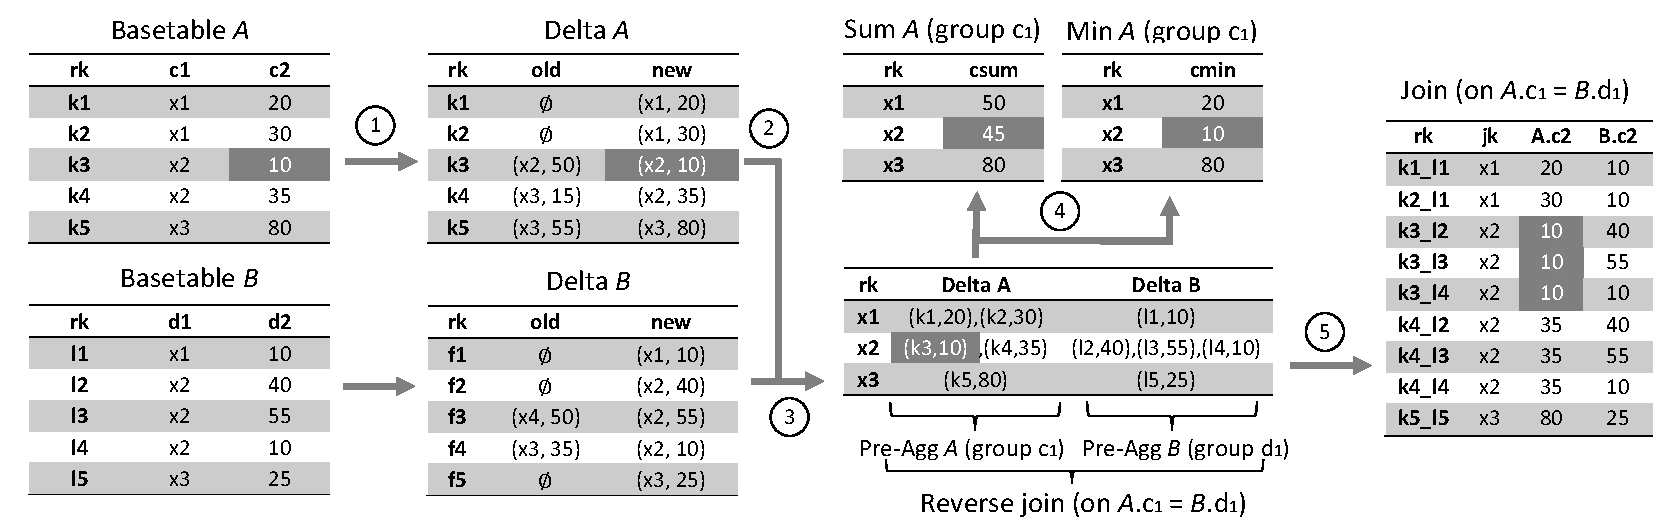
\includegraphics[width=\linewidth]{figures/ViewCalculationExample}
  \caption{View table example}\label{fig:view_table_example}
\endminipage\hfill
\vspace{-2mm}  
\end{figure*}

\noindent  
\textbf{Delta} -- The \texttt{DELTA} view is an auxiliary view that
tracks base table changes between successive update operations.  
\TL\ entries only contain the client operation.
They do not characterize the base record state before or after the
operation. For example, for a delete operation, the client only provides
the row key, but not the associated value to be deleted, as input.
Likewise, an update operation provides the row key and new values, but
not the old values to be modified. In fact, a \TL\ entry does not
distinguish between an insert and update operation. However, for view 
maintenance, this information is vital. This motivated us to introduce 
the \texttt{DELTA} view. It records base table entry changes, tracking 
the states between entry updates, i.e., the ``delta'' between two 
successive operations for a given row.  Views that derive, have this 
information available for their maintenance operations.

\noindent  
\textbf{Pre-Aggregation} -- The \texttt{PRE-AGGREGATION} view is an
auxiliary view that prepares for aggregation by sorting and grouping
base table rows. Subsequently, aggregation views only need to apply
their aggregation function to the pre-computed state. This majorly
benefits applications that calculate different aggregations over the
same aggregation key.
%
% aj - check next sentence - we mean to say w/o P-A, VMS would ...,
%      right???
%    - just a note: we could show this benefit experimentally;
%      not important right now
%
To materialize these aggregates without our pre-aggregation,
\VMS\ would have to fetch the same record over and over. Moreover, for
\texttt{MIN} and \texttt{MAX} views, the deletion of the minimum
(maximum) in the view would require an expensive base table scan to
determine the new minimum (maximum), introducing consistency issues
that result from the sought after value changing while a scan is in
progress, shown by the analysis in~\cite{jacobsen:viewmaintenance}.
This motivated us to introduce the \texttt{PRE-AGGREGATION} view. This
view type sorts the base table records according to the aggregation
key, storing the grouped rows in a map. Aggregation functions like
\texttt{COUNT}, \texttt{SUM}, \texttt{MIN}, \texttt{MAX} or
\texttt{AVG}, can then be applied to the map. Thus, aggregation
results become available instantaneously.

\noindent  
\textbf{Reverse Join} -- A \texttt{REVERSE-JOIN} view is an
auxiliary view that supports the efficient and correct materialization
of join views in \VMS.  A \texttt{JOIN} view is derived from at least two
base tables. For an update to one of these tables, the \VM\ needs to
query the other base table to determine the matching join rows. Only
if the join-attribute is the row key of the queried base table, can
the matching row be determined quickly, unless of course, an index is
defined on the join-attribute for the table.  Otherwise, a scan of the
entire table is required, which has the following drawbacks: (i) Scans
require a disproportional amount of time, slowing down view
maintenance. Also, with increasing table size, the problem worsens. (ii)
Scans keep nodes occupied, slowing down client requests.  (iii)
While a scan is in progress, underlying base tables may change, thus,
destroying view data consistency for derived views. To address these 
issues, we introduce the \texttt{REVERSE-JOIN} view.

We take the \textit{join key} ($jk$) of the two base tables as row key
of the \texttt{REVERSE-JOIN} view. When updates are propagated, the
\texttt{REVERSE-JOIN} view can be accessed from either side of the
relation with the help of the join key (it is always included in both
tables' updates). If a record is inserted into one of the underlying
base tables, it is stored in the \texttt{REVERSE-JOIN} --- whether or
not it has a matching row in the other base table.

This technique enables \texttt{INNER}, \texttt{LEFT}, \texttt{RIGHT},
and \texttt{FULL} joins to derive from the \texttt{REVERSE-JOIN} view
without the need for base table scans, as we show below.



\subsection{Standard views}
\label{subsec:common_views}

In this section, we describe how \VMS\ maintains client-exposed views
for a number of interesting standard view types. We also present
alternative maintenance strategies, but defer a full-fledged
analytical cost analysis to future work.

\noindent  
\textbf{Selection and Projection} -- A \texttt{SELECTION} view selects
a set of records from a base table based on a \textit{selection
  condition}. A \texttt{PROJECTION} view selects a set of columns from a base
table. Similar to the \texttt{SELECTION} view, the \VM\ uses the row
key of the base table as row key for the view table. To save storage and 
computation resources, we can combine \texttt{DELTA}, \texttt{PROJECTION} and
\texttt{SELECTION} into a single view. This would reduce the amount of
records (due to selection), the amount of columns (due to projection),
and still provide delta information to subsequent views. These
considerations are important for multi-view optimizations with \VMS,
which we defer to future work.

\noindent  
\textbf{Aggregation} -- The maintenance of \texttt{COUNT} and
\texttt{SUM} views is similar, so we treat them together.
Generally speaking, in aggregation views, records identified by an
\textit{aggregation key} aggregate into a single view table record.
The aggregation key becomes the row key of the view. 

\texttt{MIN} and \texttt{MAX} views are
also aggregates. Both can be derived from a \texttt{DELTA} or a
\texttt{PRE-AGGREGATION} view. When derived from a \texttt{DELTA}
view, \texttt{MIN} and \texttt{MAX} are computed similar to a
\texttt{SUM}. However, a special case is the deletion of a minimum
(maximum) in a \texttt{MIN} (\texttt{MAX}). In that case, the new
minimum (maximum) has to be determined. Without auxiliary views, a
table scan would have to be
performed~\cite{jacobsen:viewmaintenance}. This motivated us to derive
the \texttt{MIN} (\texttt{MAX}) from a \texttt{PRE-AGGREGATION}, which
prevents the need for a scan.

\noindent
\textbf{Index} -- \texttt{INDEX} views are important to provide fast
access to arbitrary columns of base tables. The view table uses the
chosen column as row key of the view, storing the corresponding table
row keys in the record value. If the client wishes to retrieve a base
table row by the indexed column, it accesses the \texttt{INDEX} view
first, then, it accesses the base table with the row keys retrieved
from the record found in the view. This is a fast type of access, for
the client is always accessing single rows by row key. 
%The
%\texttt{INDEX} view is a special case of the \texttt{PRE-AGGREGATION}
%view. If the indexed key is the same as the aggregation key, we can
%combine both view types. Further, the \texttt{PRE-AGGREGATION} can be
%combined with a \texttt{REVERSE-JOIN} view (see description above).
%Thus, we receive three different view types at the cost of one.

\noindent
\textbf{Join} -- A \texttt{JOIN} view constitutes the result of
joining $n$ base tables. Since the matching of join partners is
already accomplished by the associated \texttt{REVERSE-JOIN}, the
actual \texttt{JOIN} simply serves to combine the results in the
correct way.  To obtain the join result,
%
% aj - below - ``output operations'' is not clear
%              ``multiplies column families'' is not clear
%               Try to explain this more clearly.
%
the update program takes the output operations of the
\texttt{REVERSE-JOIN} and multiplies their column families. In this
manner, the \texttt{INNER}, \texttt{LEFT}, \texttt{RIGHT}, and
\texttt{FULL} join can be maintained, easily. So far, we are only 
providing equi joins. Theta joins, with more complex join predicates
are deferred to future work.



\subsection{View composition}
\label{subsec:view_chain}


Figure~\ref{fig:view_table_example} gives a comprehensive example of
the introduced view types (standard and auxiliary). On the left side,
two base tables $A$ and $B$ are shown. Both base tables consist of a
row key ($rk$) and two columns ($c_1, c_2$). Either base table is
connected to a delta table (Delta $A$ and $B$) that tracks the changes
of base table columns. The delta tables are connected to a
\texttt{PRE-AGGREGATION} and a \texttt{REVERSE-JOIN}, respectively.
These views reorder and group the base table records according to a
secondary key (found in columns $A.c_1$ and $B.c_1$)\footnote{One may argue
that groups of such an aggregation tend to grow very large (if
the total number of aggregation keys is small). However, due to the
column-oriented storage format of many \KVS, the values are stored
consecutively and indexed by column key -- the access still remains
fast.}.

%
% aj - above - ``column-oriented storage format'' has not been 
%              discussed in our background, has it? Or, we may add
%              a footnote to qualify/explain a bit more.
%
In the set-up of Figure~\ref{fig:view_table_example}, aggregation key
(of \texttt{SUM} and \texttt{MIN}) and join key (of \texttt{JOIN}) are
equal, so the \texttt{PRE-AGGREGATION} becomes a subset of the
\texttt{REVERSE-JOIN}. This is a good example of how a single
auxiliary view can feed multiple different views to reduce the overall
cost. The column set ($\{\}_A$) in the \texttt{PRE-AGGREGATION} serves
to directly determine the values of \texttt{SUM} and
\texttt{MIN}. Further, the cross-product of column sets $\{\}_A$ and
$\{\}_B$ serves to maintain the \texttt{JOIN} at the right side of the
figure.

The grey arrows in Figure~\ref{fig:view_table_example} depict the
paths along which the client operations are propagated to update the
view composition.  Instead of re-computing the complete views, just
the affected parts are modified. To further reduce overhead, \VMS\ 
can execute updates on single view column values; the rest of the row 
remains unaltered. 

%
% aj - below - I have a bit diffuclty understanding the below
%              also, we speak of row / column key; I believe, this
%              has not been discussed in Background
%
\textit{Example:} Now, we show a put operation that triggers a number
of updates along the view composition (see
Figure~\ref{fig:view_table_example}, the dark grey boxes): (1) The put
operation changes the value of row $k_3$, column $c_2$ in base table
$A$ from $50$ to $10$. (2) The change is propagated and represented in
Delta $A$ as $50\rightarrow 10$. (3) The corresponding column in the
\texttt{PRE-AGGREGATION} view (i.e., row key $x_2$, column
$\{c_1\}_A$) is updated. (4) This causes the sum and minimum of row
key $x_2$ in the \texttt{SUM} and \texttt{MIN} to be re-evaluated. (5)
Further, the corresponding entries in \texttt{JOIN} are updated to the
new value $10$. As depicted, \VMS\ always accesses a single column
value (to update the view tables); the access is executed with
knowledge of row and column key. Since a \KVS\ guarantees fast row and
column key access, -- actually, this is what they are built for, --
the update propagates rapidly through the composition.  Besides the
example in Figure~\ref{fig:view_table_example}, more complex view
compositions can be created by combining different types of view
tables.

% aj - This is a bit strong. SQL is a very complex language; VMS does
%      support full fledged SQL somebody could argue
%
%... such that any kind of SQL-query can be expressed.
%








 










%\subsection{Proof of Consistency}


Theorem~\ref{theo:strong_consistency} states that a VMS system fulfilling all 
three requirements achieves at least strong consistency. In the following, we 
will present a proof for this theorem, which is organized in three stages: we 
start with proving convergence and then present extensions to also prove weak 
consistency  and finally strong consistency.





\subsubsection{Notation}
First, we define the following notation for keys, 
operations on keys, and the ordering of operations. Let $k_x$ denote a key in 
a base table, where $x \in X = \{1, \dots, m\}$, and $X$ is the 
table's key range. Further, let an operation on key $k_x$ be defined as 
$t[k_x]$, and a totally ordered sequence of such operations be denoted by 
$\langle t_1, t_2, t_{3}, \dots, t_N\rangle$, where $N$ defines the total 
number of operations on the table in a given timespan. 
Hence, a generalized sequence of operations on a base table is 
represented by $\langle t_1[k_{x_1}], t_2[k_{x_2}], \dots, 
t_n[k_{x_m}]\rangle$, where $k_{x_1}, \dots, k_{x_m} \in X$ can be arbitrarily 
chosen from the base table's key range for every timestamp. Based on this 
generalized sequence every other sequence of operations can be derived, e.g. 
$\langle t_1[k_{1}],t_2[k_{2}],t_3[k_{1}]\rangle$. In some cases, we also want 
to keep the ordering of operations variable. For that reason, we introduce an 
index $s_i$ with $i \in \{1, \dots, n\}$. Then we can write the arbitrary 
sequence as $\langle t_{s_1}[k_{x_1}], t_{s_2}[k_{x_2}], \dots, 
t_{s_n}[k_{x_n}]\rangle$ with $s_1\neq \dots \neq s_n$. Using this notion, we 
are capable of representing every possible sequence of update operations in 
the system. 

The index $t^{(i)}[k_x]$ is used to express a sequence of operations on 
a single row key (i.e. the time-line). For example, a sequence of 
operations on row key $k_x$ is denoted as $\langle 
t^{(1)}[k_x],t^{(2)}[k_x]...,t^{( \omega)}[k_x]\rangle$. The last 
operation on a particular row key is always denoted with $\omega$. (see 
Section~\ref{sec:consistency}).

For the proof, we assume such an arbitrary sequence of base table operations
 and then we show that --- given the requirements in the theorem --- a VMS 
 system will produce correct view results. Formally, we show that $V_f=View(B_f)$. 

\subsubsection{Convergence}
\label{sub:proof_convergence}
As mentioned earlier, every view type defines its own mapping from base table 
to view table records. Thus, we prove the different cases separately. 

\noindent
\textit{One-to-one mapping:} \texttt{SELECTION}, \texttt{PROJECTION} 
views define a one-to-one mapping between base and view table. The row 
key of the base table is also the row key of the view table. Operations 
for both view types are idempotent, meaning an operation could be 
applied several times without changing the result. The view record is 
always a representation of the last base table operation applied. A 
correct view record with row key $k$ is defined as the last operation on 
the row key in the base table key, e.g. $k\leftarrow 
View(t^{(\omega)}[k])$. The function $View$ calculates the view record 
(by using the appropriate view definition) and applies the result to the 
correct view key. A view table converges, if all view records are 
computed correctly in the last view state. 

We start defining an arbitrary sequence of operations on the base table, 
shown in Step~\ref{proof:oo_step1}. Clients can update different row 
keys in the base table, using put or delete operations. Likewise, they 
can update the same row key multiple times. The update operations of the 
clients form a particular global order, expressed through $t_1..t_n$. 
They take the base table from its initial state $B_0$ to its final state 
$B_f$. In the next step, all update operations get forwarded, causing 
the ordering of operations to be lost. If we would continue working with 
an unordered set, convergence of the view will be violated at some 
point. For this reason, we apply requirement (iii) (,i.e. the time-line 
requirement) to our equation, as depicted in Step~\ref{proof:oo_step3}. 
As updates operations do not influence each other (see requirement 
(ii)), we are able to create a set of sub-sequences. These 
sub-sequences only consist of updates that have been applied to the same 
row key. Likewise the sub-sequences contain all operations from the 
previous step (see requirement (i)). 
%
\begin{subequations}
  \begin{align}
 S_b&=\langle t_1[k_{x_1}],....,t_n[k_{x_n}] \rangle;\;\;\Big(B_0 \overset{S_b}{\rightarrow}B_f\Big) \label{proof:oo_step1}\\ 
 S_1&=\langle t^{(1)}[k_{1}],..,t^{(\omega_1)}[k_{1}]\rangle,..,S_m=\langle t^{(1)}[k_{m}],..,t^{(\omega_m)}[k_{m}]\rangle\label{proof:oo_step3}\\
  S_1&=\langle t^{(\omega_1)}[k_{1}]\rangle,..,S_m=\langle t^{(\omega_m)}[k_{m}]\rangle\label{proof:oo_step4}\\
 S_v&=\langle t_{s_1}^{(\omega_1)}[k_{1}],..t_{s_n}^{(\omega_m)}[k_{m}]\rangle;\; \Big(V_0\overset{S_v}{\rightarrow}V_f\Big)\label{proof:oo_step5}\\
 	V_f&=k_x\leftarrow View(t^{(\omega_x)}[k_x])=View(B_f)\label{proof:oo_step6}
  \end{align}
\end{subequations}
%
In Step~\ref{proof:oo_step4}, we pick the last element of all 
sub-sequences and eliminate the rest. As stated above, only the last 
operation on a particular row key has an influence on the final view 
state. Again, we observe that the time-line of a row key is vital. If it 
is broken, e.g. for row key $k_1$, then an operation 
$t^{(\omega-1)}[k_{1}]$ can be incorporated into the final result and 
render it incorrect. After the elimination, we unite the operations 
again in Step~\ref{proof:oo_step5}. The reunion allows the remaining 
operations to be executed in every possible order (i.e. every operation 
could be executed in parallel). Finally, the view definition is applied 
to every operation in $R$. This leads to the correct final view records 
and hence, to convergence. The \texttt{DELTA} view also defines a 
one-to-one mapping between base and view records. In contrast to the 
aforementioned views, the results of the \texttt{DELTA} view do not only 
relate to the last, but to the two last operations. Therefore, we need 
to change the last three steps of the proof as follows: 
%
\begin{subequations}
  \begin{align}
  S_1&=\langle t^{(\omega_1-1)}[k_{1}],t^{(\omega_1)}[k_{1}]\rangle,..,S_m=\langle t^{(\omega_m-1)}[k_{m}],t^{(\omega_m)}[k_{m}]\rangle\\
   S_v&=\langle t_{s_1}^{(\omega_1-1)}[k_{1}],t_{s_2}^{(\omega_1)}[k_{1}],..t_{s_{n-1}}^{(\omega_m-1)}[k_{m}],t_{s_n}^{(\omega_m)}[k_{m}]\rangle\label{proof:ood_step2}\\
   &(\forall t_{s_i}^{(\omega_y-1)}\in S_v)(\exists t_{s_j}^{(\omega_y)}\in S_v)\;s_i < s_j;\;\Big(V_0\overset{S_v}{\rightarrow}V_f\Big)\notag\\
 	V_f&=k_x\leftarrow View(t^{(\omega_x-1)}[k_x],t^{(\omega_x)}[k_x])=View(B_f)
  \end{align}
\end{subequations}
%
As can be observed in Step~\ref{proof:ood_step2}, the two last 
operations of a time-line are included into the final result. However, 
the sequence can be arbitrarily ordered, but needs to preserve the 
time-line of both last operations (i.e. $\omega-1$ must always precede 
$\omega$). Computing $V_f$ leads to the valid final state and the 
\texttt{DELTA} view converges. 

\noindent
\textit{Many-to-one mapping:} (\texttt{PRE}-)\texttt{AGGREGATION} and 
\texttt{INDEX} views define a many-to-one mapping between base and view 
table. The row key of the view table is the aggregation key. Multiple 
row keys in the base table can relate to a particular aggregation key. 
However, a base table row has always only one aggregation key. A correct 
view record with aggregation key $x$ is defined as the combination of 
multiple base records $k_{x_1}..k_{x_j}$, related to the particular key. 
In terms of incremental view maintenance, the correct view record can be 
defined as a number of last operations, that have been applied to this 
combination of base records: $x \leftarrow 
View(t^{(\omega_1)}[k_{x_1}],..,t^{(\omega_j)}[k_{x_j}])$. In case of a 
\texttt{SUM} view e.g., this resolves to $x \leftarrow 
f(t^{(\omega_1)}[k_1])+..+f(t^{(\omega_j)}[k_j])$. We start again, 
defining an arbitrary sequence of base table operations in 
Step~\ref{proof:mo_step1}. In contrast to the previously handled views, 
we are now processing $\delta$-operations. We construct a number of $m$ 
sub- sequences, each containing the $\delta$-operations of one 
particular base record key. In Step~\ref{proof:mo_step2}, we merge the 
$\delta$-operations together. All $\delta$- operations add up to form 
the last transaction as the end result (i.e. $\delta(t^{(1)}[k_{1}])+
..+\delta(t^{( \omega_1)}[k_{1}])=t^{(\omega_1)}[k_{1}]$). 
%\begin{subequations}
%  \begin{align}
%  \{t_1(k_1),..,t_n(k_1)..t_1(k_n),..,t_n(k_n)\}\\
% \{\langle t_1(k_1),..,t_n(k_1)\rangle,..\langle t_1(k_n),..,t_n(k_n)\rangle\}\\
% \{\langle t_n(k_1)\rangle,..\langle t_n(k_n)\rangle\}\\
% 	x=f(t_n(k_1))+..+f(t_n(k_n))
%  \end{align}
%\end{subequations}
%
\begin{subequations}
  \begin{align}
  S_b&=\langle t_1[k_{x_1}],....,t_n[k_{x_n}] \rangle;\;\Big(B_0 \overset{S_b}{\rightarrow}B_f\Big) \label{proof:mo_step1}\\ 
 S_1&=\langle \delta(t^{(1)}[k_{1}]),.,\delta(t^{(\omega_1)}[k_{1}])\rangle,..,\label{proof:mo_step2}\\
 &\hspace{10 mm}S_m=\langle \delta(t^{(1)}[k_{m}]),.,\delta(t^{(\omega_m)}[k_{m}])\rangle\notag\\
  S_1&=\langle t^{(\omega_1)}[k_{1}]\rangle,..,S_m=\langle t^{(\omega_m)}[k_{m}]\rangle\\
 S_v&=\langle t_{s_1}^{(\omega_1)}[k_{1}],..t_{s_n}^{(\omega_m)}[k_{m}]\rangle;\;\Big(V_0\overset{S_v}{\rightarrow}V_f\Big)\label{proof:mo_step4}\\
 	V_f&=x\leftarrow View(t^{(\omega_{x_1})}[k_{x_1}],.., t^{(\omega_{x_j})}[k_{x_j}])=View(B_f)\label{proof:mo_step5}
 	%&\hspace{10 mm}x_1,..,x_j \in \{1,..,m\};\;x_1\neq,..,\neq x_j \notag
  \end{align}
\end{subequations}
%
Now, we can unite the single sequences as done before. We retrieve a 
final sequence as shown in Step~\ref{proof:mo_step4}. The operations of 
this sequence are then applied to the view --- simultaneously they are 
grouped and stored according to their aggregation key. The final view 
records are calculated correctly, as depicted in 
Step~\ref{proof:mo_step5}, which causes the aggregation view to 
converge. 

\textit{Many-to-many mapping:} (\texttt{REVERSE}-)\texttt{JOIN} views 
define a many-to-many mapping between base and view table. The row key 
of the view table is a composite key of both join tables' row key. 
Multiple records of both base tables form a set of multiple view records 
in the view table. Since the joining of tables takes place in the 
\texttt{REVERSE JOIN} view, we prove convergence only for this view 
type. A \texttt{REVERSE JOIN} view has a structure that is similar to an 
aggregation view. The row key of the \texttt{REVERSE JOIN} view is the 
join key of both tables. All base table records are grouped according to 
this join key. But in contrast to an aggregation view the 
\texttt{REVERSE JOIN} view combines two base tables to create one view 
table. A correct view record with join key $x$ is defined as a 
combination of operations on keys $k_1..k_n$ from join table $A$ and 
operations on keys $l_1..l_p$ from join table $B$. In order to represent 
both keys we introduce an additional variable $z_1,..,z_n \in 
\{k_1,..,k_m, l_1,..,l_p\}$. Then, the correct view record is defined 
as: $x \leftarrow View(t^{(\omega_1)}[z_1], ..,t^{(\omega_j)}[z_j])$. 
We start with a sequence of arbitrary client updates to both base 
tables, as depicted in Step~\ref{proof:mm_step1}. Then, the order of 
updates is lost and the time-line requirement is realized in 
Step~\ref{proof:mm_step2}. 
%
\begin{subequations}
  \begin{align}
  S_b&=\langle t_1[z_1],..,t_n[z_n]\rangle;\;\Big(B_0 \overset{S_b}{\rightarrow}B_f\Big)\label{proof:mm_step1}\\ 
 S_1&=\langle \delta(t^{(1)}[k_{1}]),..,\delta(t^{(\omega_1)}[k_{1}])\rangle,..,S_m,..,S_{m+1},..\label{proof:mm_step2}\\ 
&\hspace{10 mm}S_{m+p}=\langle \delta(t^{(1)}[l_{p}]),..,\delta(t^{(\omega_p)}[l_{p}])\rangle\notag\\
  S_1&=\langle t^{(\omega_{k_1})}[k_{1}]\rangle,.., S_m=\langle t^{(\omega_{k_m})}[k_{m}]\rangle,..,\\
 &\hspace{10 mm}S_{m+1}=\langle t^{(\omega_{l_1})}[l_{1}]\rangle,..,S_{m+p}=\langle t^{(\omega_{l_p})}[l_{p}]\rangle\notag\\
 S_v&=\langle t^{(\omega_{k_1})}[k_{1}],..t^{(\omega_{k_m})}[k_{m}],\\
 &\hspace{10 mm}t^{(\omega_{l_1})}[l_{1}],..,t^{(\omega_{l_p})}[l_{p}] \rangle;\;\Big(V_0\overset{S_v}{\rightarrow}V_f\Big)\label{proof:mm_step3}\\
 	V_f&=x\leftarrow View(t^{(\omega_{z_1})}[z_1],.., t^{(\omega_{z_j})}[z_j])=View(B_f)\label{proof:mm_step4}
 	%&\hspace{10 mm}z_1,..,z_j \in \{k_1,..,k_m,l_1,..,l_p\}; z_1\neq,..,\neq z_j ;\; \notag
  \end{align}
\end{subequations}
%
We eliminate all but the last operations $\omega$ and reunite the 
operations in Step~\ref{proof:mm_step3}. This leads to the final 
Step~\ref{proof:mm_step4}, where the operations are applied to the view 
record. Since the view records are calculated correctly (i.e. only the 
last operations of the row keys are included) we conclude that the view 
converges. 

\subsubsection{Weak consistency} 
\label{sub:proof_weak}

Weak consistency has been defined as follows: Weak consistency is given 
if the view converges and all intermediary view states are valid, 
meaning they can be derived from one of the base states with 
$V_j=View(B_i)$. As we already proved convergence, we need show that all 
the intermediary view states are correct likewise. We start again with 
an arbitrary sequence of operations in Step~\ref{proofw:oo_step1}. In 
order to generate an intermediate base state, we cut the sequence at any 
point before an operation $t_a$, with $1 < a < n$. After the ordering is 
lost, we apply the time-line consistency. But in contrast to before, we 
are not capable of processing the complete time-line (i.e. 
$(1)..(\omega)$). Instead, we process the time-line until an 
intermediary element $\alpha_x \leq \omega_x$. 
%
\begin{subequations}
  \begin{align}
  S_b&=\langle t_1[k_{x_1}],....,t_n[k_{x_n}] \rangle;\;\Big(B_0 \overset{S_b}{\rightarrow}B_{a}\Big)\label{proofw:oo_step1}\\
 S_1&=\langle t^{(1)}[k_{1}],..,t^{(\alpha_1)}[k_{1}]\rangle,..,S_m=\langle t^{(1)}[k_{m}],..,t^{(\alpha_m)}[k_{m}]\rangle\\
 S_v&=\langle t_{s_1}^{(1)}[k_{1}],..t_{s_i}^{(\alpha_1)}[k_{1}],..,t_{s_j}^{(1)}[k_{m}],..,t_{s_a}^{(\alpha_m)}[k_{m}]\rangle;\;\Big(V_0\overset{S_v}{\rightarrow}V_a\Big)\\
 (\forall& t_{s_1}^{(\lambda_1)}[k_{x_1}] \in S_v)(\forall t_{s_2}^{(\lambda_2)}[k_{x_2}] \in S_v):(x_1=x_2)\;\land\;(\lambda_1<\lambda_2) \Rightarrow s_1 < s_2\notag\\
V_{a}&=k_x\leftarrow View(t^{(\alpha_x)}[k_x])=View(B_{\alpha})
  \end{align}
\end{subequations}


\subsubsection{Strong consistency}
\label{sub:proof_strong}

Strong consistency has been defined as follows: Weak consistency is 
achieved and the following conditions hold true. All pairs of view 
states $V_i$ and $V_j$ that are in a relation $V_i \leq V_j$ are derived 
from base states $Bi$ and $B_j$ that are also in a relation $B_i \leq 
B_j$. Since weak consistency is already proven, we only need to prove 
the statement $V_i \leq V_j \Rightarrow B_i \leq B_j$. If this statement 
is negated, then only two of the following cases can occur: Either $V_i 
\leq V_j \Rightarrow B_i \parallel B_j$ or $V_i \leq V_j \Rightarrow B_i 
\geq B_j$. Both cases can only be constructed by breaking the record 
time-line. To be precise: At least one record has to exists, whose 
time-line is broken. Formally, we demand $ (\exists t_l \in B_i)(\forall 
t_k \in B_j):(r(t_l)=r(t_k))\land(l > k) $. Because requirement (iv) 
prevents the breaking of time-lines, we conclude that both cases are not 
possible. Thus, we have proven strong consistency by contradiction. 




%\section{Fault Tolerance}
\label{sec:fault_tolerance}

Failure detection and recovery play a critical role, especially in
large-scale distributed systems.  In this section, we analyze the
behavior of VMS under VM and node crashes to ensure that after
appropriate recovery measures, views still converge.

\noindent
\textbf{VM crash} -- A VM maintains a queue with operations dispatched
to it. Upon a VM crash, these updates are lost, which may result in
non-converging views. Our recovery measures described here, ensure
view convergence under VM crash. For every update a VM propagates, it
stores the sequence ID of the processed operation in its commit log. A
VM crash triggers an event via Zookeeper
(cf. Section~\ref{sec:system_overview}), notifying the VMS
coordinator. Via the commit log, the coordinator retrieves the last
operation the crashed VM successfully propagated. The commit log order
is determined by the order the VM propagates updates, which results
from the stream of operations dispatched to it, respecting record
timeline semantics. Now, the coordinator executes the steps of
Algorithm~\ref{alg:crashed_vm}.



\begin{algorithm}
\caption{VM recovery in VMS}
\label{alg:crashed_vm}
\begin{algorithmic}[5]
\Procedure{$onVMCrashed$}{$nx, VM_{nx}, vm_c$}
\State $sendMessage(nx, withdraw, vm_c)$
\ForAll{$vm \in VM_{nx}$}	
\State $sendMessage(vm, requestSID)$
\EndFor
\ForAll{$vm \in VM_{nx}$}	
\State $SIDs \leftarrow receiveMessage(vm, SID)$	
\EndFor
\State $smallestSID \leftarrow minimum(SIDs)$
\State $sendMessage(nx, replay, smallestSeqID)$	
\EndProcedure
\end{algorithmic}
\end{algorithm}

First, the coordinator sends a withdraw command to the 
concerned NX component. The NX withdraws the crashed VM from the 
hash-ring and stops dispatching operations to it. This way no updates, 
that were in-fight while the VM crashed, are lost. Next, the coordinator 
obtains the last sequence ID of every VM (assigned to the node the 
crashed VM belonged to) and determines the smallest one, including the 
one from the crashed VM's commit log. The VMS advises the NX component 
to replay the log entries from the point of the smallest ID. This 
recovery measure is necessary for the following reasons: It might happen 
that a running view manager is executing a base table operation with a 
smaller sequence ID than the crashed one. Then, a replay from the crashed 
view manager's ID would cut off some of the client operations. Taking 
the smallest sequence ID, the VMS ensures that no operation gets lost.
However, there might be a case when the crashed view manager had already 
queued up operations but not written anything to the commit log.  Then 
the recovery of the sequence ID fails and again, operations may be lost.
The VM can just avoid this case by writing the first sequence ID it ever
receives from a node, directly to the commit log, marking it as 'not 
processed'. Then the transaction log can be replayed from this point. 
Another problem during replay is that some operations may be forwarded 
to the view managers again. This leads to duplicate view updates. 
But thanks to the signature mechanism (cf.Section~\ref{sec:consistency}), 
the duplicate operations can be identified and just ignored. 


\noindent
\textbf{Node crash} -- A node crash is handled by the recovery
mechanism of the KV-store. It selects a new node and replay's the
crashed node's TL. The coordinator of VMS just notices the
crash  and re-assigns the idle view managers to another
node.



\section{Evaluation}

\subsection{Set-up}

\subsection{Work load}

\subsection{Experiments}



%
\section{Related work}

Research of incremental view maintenance technologies started back in 
the nine-ties. The research was primarily conducted with regard to data 
warehouses \cite{warehouse1, warehouse2, warehouse3, warehouse4}. While 
many principles of incremental maintenance still apply today (e.g. how 
deltas are computed), the underlying architectures have changed 
significantly. The storage capacity has grown, the degree of 
distribution increases continuously. Even though, there was research on 
maintenance of distributed sources \cite{warehouse3}, the warehouse 
itself was a stand-alone system that could be easily queried to retrieve 
information. With the amount of analytical data today multi-view 
optimization becomes a problem. 

Cui and Widom \cite{warehouse1, warehouse2} already examined the usage 
of auxiliary views. Even if the auxiliary views in our context serve a 
different purpose (they define a pre-step of the logical computation), 
they materialized intermediate steps to save processing effort. Already 
here the trade-off of storage vs. processing capacity can be observed. 
However, their research \cite{warehouse1, warehouse2} was more related 
to the problem of lineage tracing and view selection. 

View selection as is also described in \cite{view_selection1, 
view_selection2} is problem, where an algorithm decides, which sub-set 
of a set of view candidates should be materialized. Especially in the 
context of multi-query optimization \cite{multi_query1, multi_query2, 
multi_query3, multi_query4, multi_query5}, it is widely used. However, 
view selection is a different problem than multi-view optimization 
(especially views that are maintained incrementally). In multi-view 
optimization every view has to be materialized. The problem is not the 
choice of the correct materialization set-up, but the reduction of 
processing and storage capacity by resource sharing. 

Even if not the same problem, multi-query optimization (or view 
selection) can provide instruments to also approach the multi-view 
problem. For example, the maintenance plan (e.g. the AND-OR query DAG) 
or a cost model, similar to that of the Volcano optimizer 
\cite{multi_query4, multi_query5} can be used to find an optimal 
solution for the multi-view problem. 

A lot of the modern algorithms for sharing results and optimizing in a 
multi-query environment are based on the map-reduce paradigm 
\cite{map_reduce1, map_reduce2, map_reduce3, map_reduce4}. Map-reduce 
provides a very similar data model to our solution -- records are 
processed in a key-value format. The translation of SQL-statements into 
basic expressions (like selection, aggregation, join) that can share 
elements of computation \cite{map_reduce3} is somewhat comparable to our 
solution. However, the processing style for map-reduce is a 
batch-oriented strategy. Self-contained sets of records are retrieved, 
computed and stored back to disk. When discussing the sharing of 
intermediate results, this problem also reduces to a view selection 
problem. As already stated, our model favours an incremental strategy.
As we are dealing with streams of transactions (as opposed to sets of 
records), optimization algorithms are different. 




%
\section{Conclusions}
\label{sec:conclusion}

In this paper, we developed a scalable view maintenance system, fully 
integrated with a distributed KV-store. We demonstrated the 
efficient, incremental, and deferred materialization of selection, 
index, aggregation, and join views with HBase. Our approach is capable 
to consistently maintain multiple views that may depend on each other. 
In the spirit of KV-stores, our view maintenance architecture is 
incrementally scalable by adding additional view managers as maintenance 
load increases. In our approach, a stream of base table updates is 
propagated to view tables by a bank of view managers operating in 
parallel. To establish view table consistency, we resort to the 
application of a number of known techniques that are combined in novel 
ways to materialize views consistently. We also address fault tolerance 
and recovery to react to failing view managers in our approach. Our 
experimental evaluation quantified the benefits and cost of the approach 
and shows that it scales linearly in view update load and number of view 
managers running. 

In future work, we aim at exploring optimizations for the maintenance of 
multiple, overlapping view expressions and explore automatic means for 
reacting to view maintenance load variations in our architecture. 

% The following two commands are all you need in the
% initial runs of your .tex file to
% produce the bibliography for the citations in your paper.
\bibliographystyle{abbrv}
\bibliography{vldb_sample}  % vldb_sample.bib is the name of the Bibliography in this case
% You must have a proper ".bib" file
%  and remember to run:
% latex bibtex latex latex
% to resolve all references
%
%\subsection{References}
%Generated by bibtex from your ~.bib file.  Run latex,
%then bibtex, then latex twice (to resolve references).

%APPENDIX is optional.
% ****************** APPENDIX **************************************
% Example of an appendix; typically would start on a new page
%pagebreak

%\begin{appendix}
%You can use an appendix for optional proofs or details of your evaluation which are not absolutely necessary to the core understanding of your paper. 
%
%\section{Final Thoughts on Good Layout}
%Please use readable font sizes in the figures and graphs. Avoid tempering with the correct border values, and the spacing (and format) of both text and captions of the PVLDB format (e.g. captions are bold).
%
%At the end, please check for an overall pleasant layout, e.g. by ensuring a readable and logical positioning of any floating figures and tables. Please also check for any line overflows, which are only allowed in extraordinary circumstances (such as wide formulas or URLs where a line wrap would be counterintuitive).
%
%Use the \texttt{balance} package together with a \texttt{\char'134 balance} command at the end of your document to ensure that the last page has balanced (i.e. same length) columns.
%
%\end{appendix}



\end{document}
